\documentclass[11pt]{article}

% 页面设置
\usepackage[top=1cm, bottom=2cm, left=1cm, right=1cm]{geometry}

% 中文支持
\usepackage{ctex}

% 数学包
\usepackage{amsmath, amssymb, amsthm}

% 算法包
\usepackage[linesnumbered, ruled]{algorithm2e}

% 颜色和命令定义
\usepackage{xcolor, xparse}

% 代码显示
\usepackage{listings}

% 图形包
\usepackage{graphicx}

% 子图包
\usepackage{subcaption}

% 表格包
\usepackage{booktabs}

% 其他需要的包
\usepackage{mathrsfs}
\usepackage{wrapfig}
\usepackage{forest}
\usepackage[normalem]{ulem} % 保持 \emph 为斜体
\usepackage{bm}
\usepackage{multicol}
\usepackage{verbatim}
\usepackage{float}
\usepackage{pifont}
\usepackage{enumitem} % 使用更多的列表标签
\usepackage[hypcap=false]{caption}


% 添加 'soul' 包用于高亮和支持换行
\usepackage{soul}

% 定义自定义颜色
\definecolor{cmdbg}{RGB}{220, 220, 220} % 浅灰色背景

% 设置高亮颜色
\sethlcolor{cmdbg}

% 定义 \ccmd 命令,用于行内代码片段
\newcommand{\ccmd}[1]{\texttt{\hl{#1}}}

% 超链接(放在最后)
\usepackage[colorlinks=true, linkcolor=blue]{hyperref}

\author{
    \makebox[0.8\textwidth]{%
        \centering
        杨远青 \quad 22300190015 \quad
        \href{https://github.com/bud-primordium/pytorch_exercise/tree/main/AI_Phys_Hw_2}{\raisebox{-2pt}{
\includegraphics[height=12pt]{comphys.pdf}}}
    }
}



\title{基于M\"{u}ller--Brown势的神经网络建模\\}

\begin{document}
\maketitle
% \textit{正面迎击ddl军团!}


\section{问题描述}
\subsection{函数定义}
M\"{u}ller--Brown势能函数解析式为:
\[
    U(x_1, x_2) = s \cdot \sum_{k=1}^4 A_k \exp\left[
        \alpha_k (x_1 - a_k)^2 + \beta_k (x_1 - a_k)(x_2 - b_k) + \gamma_k (x_2 - b_k)^2
        \right]
\]
\subsection{参数系统}
\begin{minipage}[t]{0.45\textwidth}
    \vspace{-\baselineskip}
    \begin{align*}
        \text{振幅系数:}  & \quad \bm{A} = (-200, -100, -170, 15)       \\
        \text{二次项参数:} & \quad
        \begin{aligned}[t]
            \bm{\alpha} & = (-1, -1, -6.5, 0.7)   \\
            \bm{\beta}  & = (0, 0, 11, 0.6)       \\
            \bm{\gamma} & = (-10, -10, -6.5, 0.7)
        \end{aligned}                       \\
        \text{中心坐标:}  & \quad
        \begin{aligned}[t]
            \bm{a} & = (1, 0, -0.5, -1) \\
            \bm{b} & = (0, 0.5, 1.5, 1)
        \end{aligned}                                 \\
        \text{缩放因子:}  & \quad s = 0.05                              \\
        \text{定义域:}   & \quad x_1 \in (-1.5,1.5),\ x_2 \in (-0.5,2) \\
        \text{势能截断:}  & \quad U \leq  U_{\text{cut}} = 9            \\
    \end{align*}
\end{minipage}
\hfill
\begin{minipage}[t]{0.48\textwidth}
    \vspace{-\baselineskip}
    \centering
    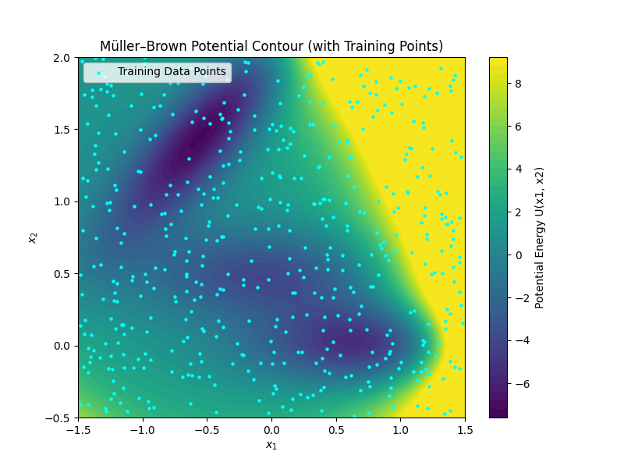
\includegraphics[width=\linewidth]{potential_data.png}
    \captionof{figure}{待拟合势能面与训练集可视化}
    \label{fig:surface}
\end{minipage}
\subsection{评估标准}
MAE\footnote{最终MAE系列评价指标分为:全局MAE、训练集MAE、测试集MAE,其中全局MAE\textbf{不是}训练集和测试集的MAE的加权平均值,而是在全势能面上采集的($100\times100$)个点(相当于更大的超测试集),与受限于优化采点策略的训练集、测试集,略有不同。}:
\[
    \text{MAE} = \frac{1}{N} \sum_{i=1}^N |U(x_1^{(i)}, x_2^{(i)}) - U_{\text{NN}}(x_1^{(i)}, x_2^{(i)})|
\]


及训练时间等。

\section{模型设计}

\begin{figure}[H]
    \centering
    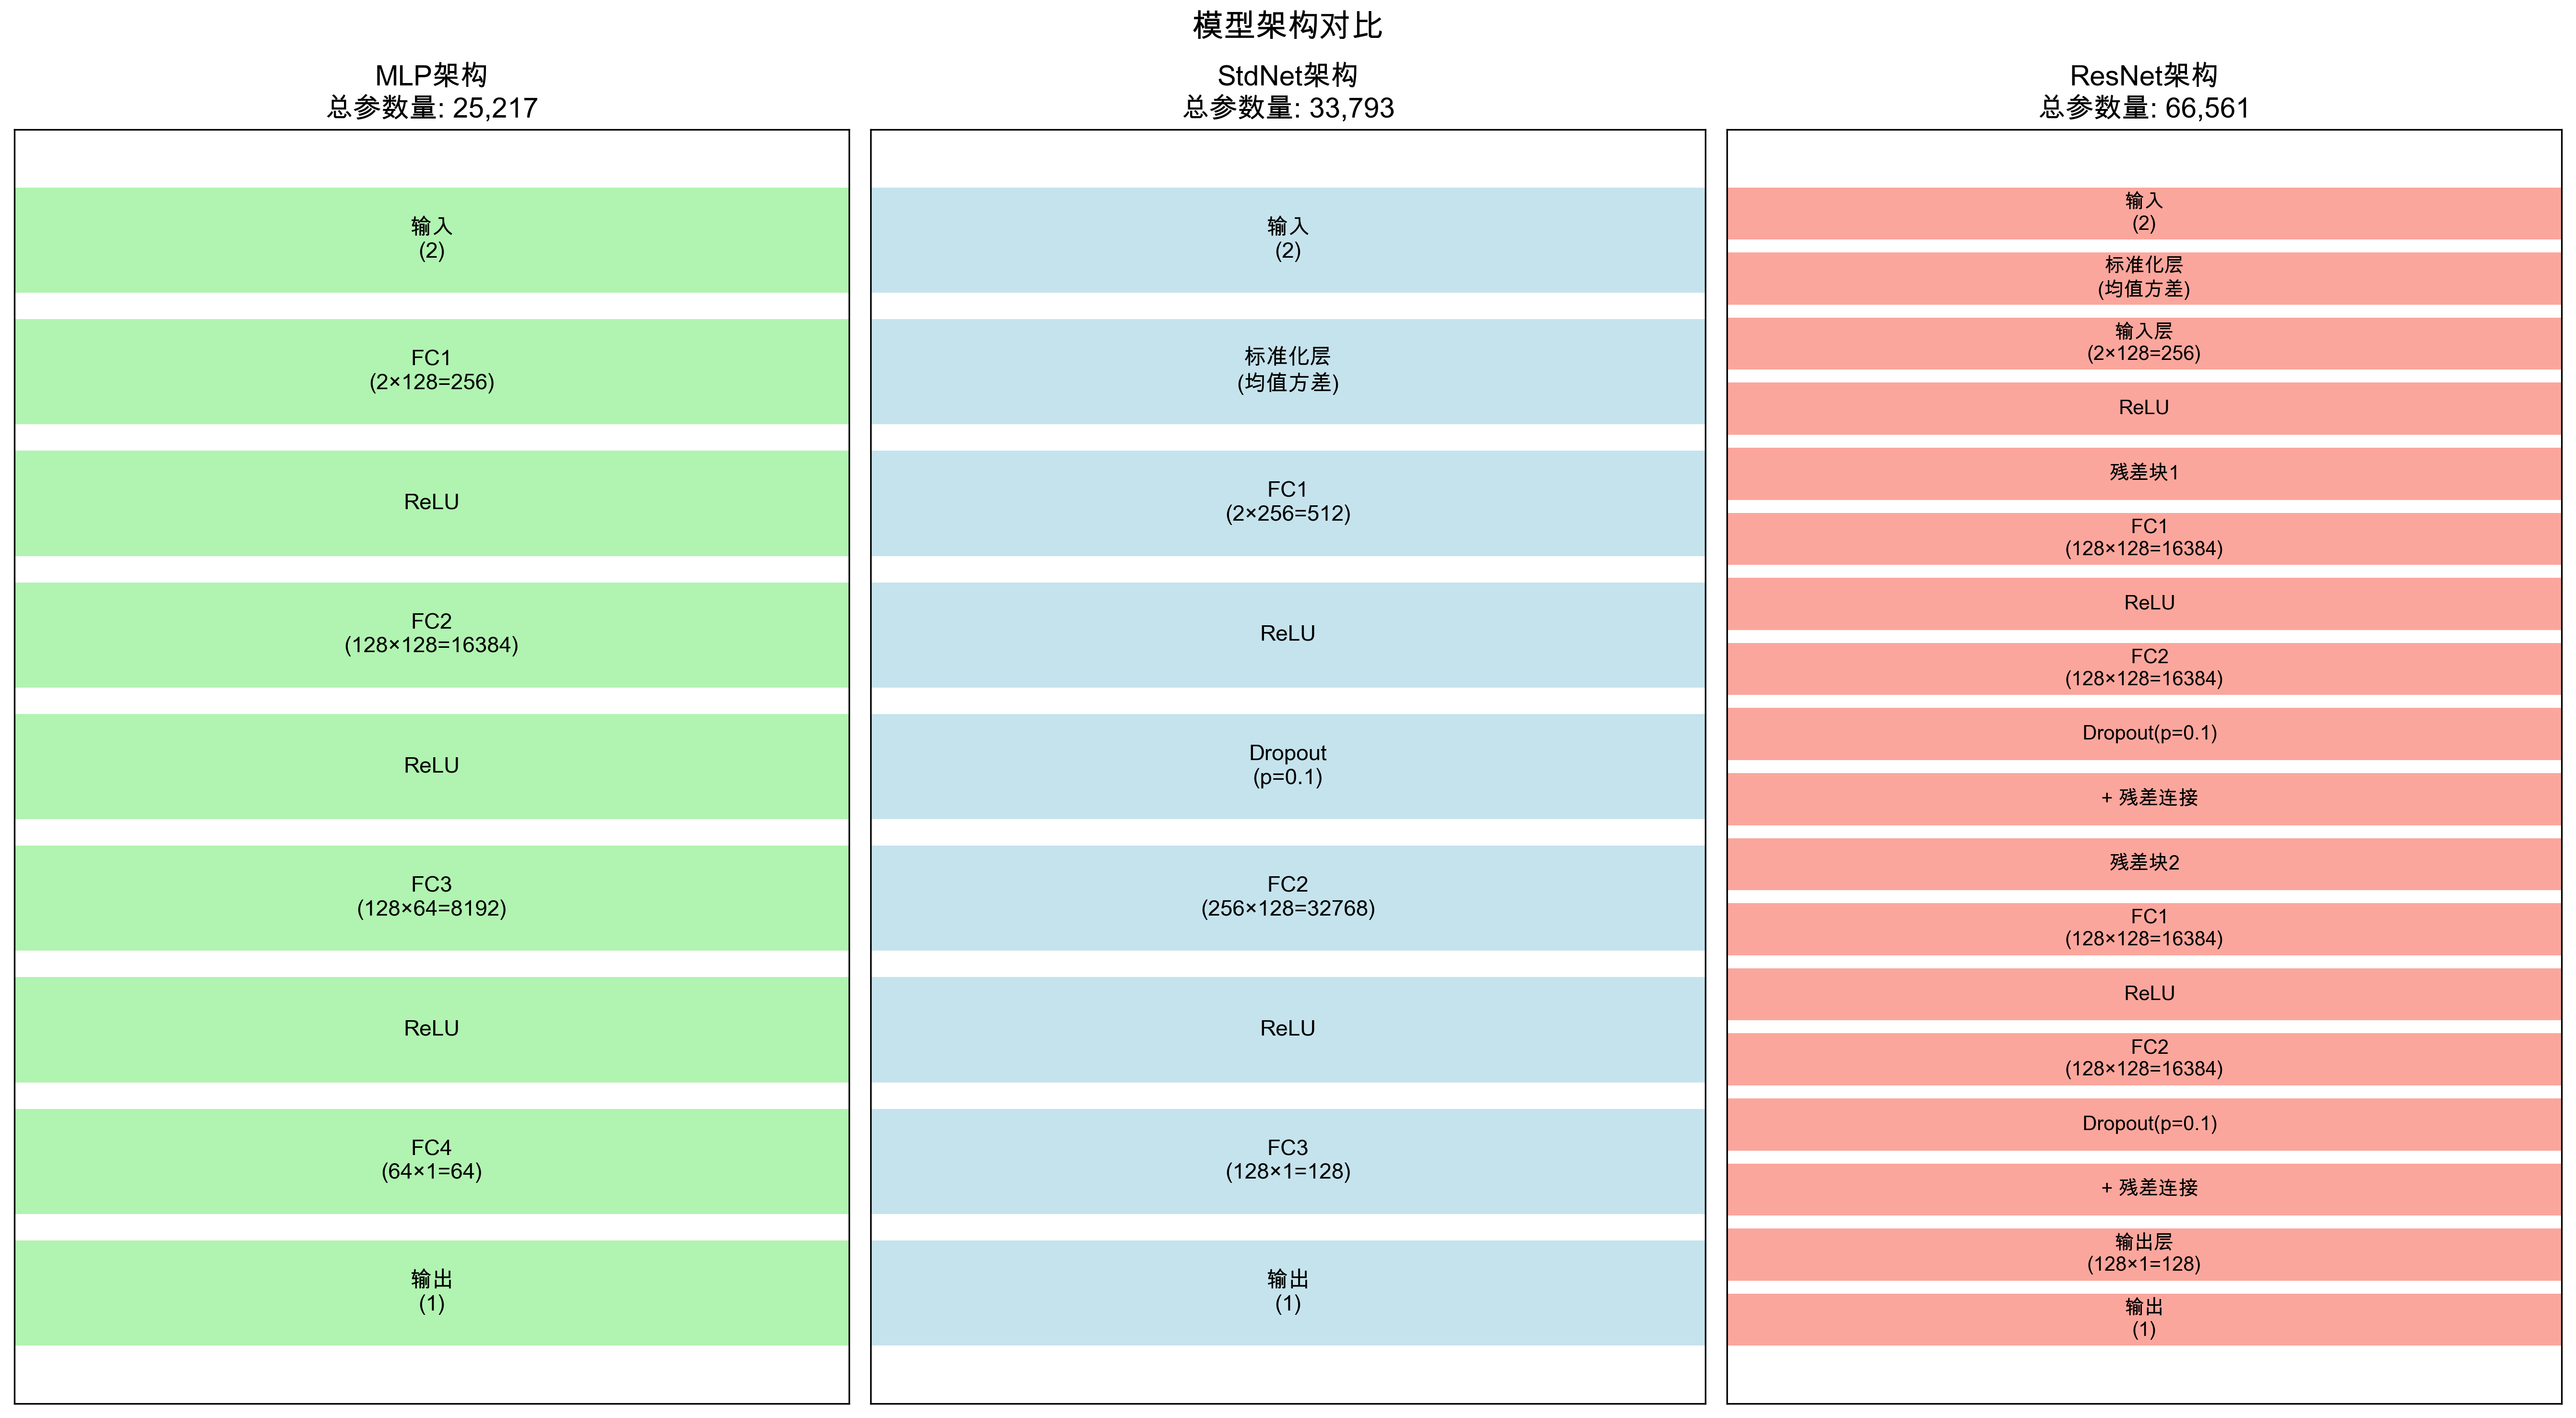
\includegraphics[width=0.9\linewidth]{results_20250330_150206/figures/模型架构对比.png}
    \caption{三种神经网络模型架构对比}
    \label{fig:model_comparison}
\end{figure}

\subsection{MLPNet}
\begin{align*}
    \mathbf{h}_1              & = \text{ReLU}^\dagger(\mathbf{W}_1 \mathbf{x} + \mathbf{b}_1) \in \mathbb{R}^{128} \\
    \mathbf{h}_2              & = \text{ReLU}(\mathbf{W}_2 \mathbf{h}_1 + \mathbf{b}_2) \in \mathbb{R}^{128}       \\
    \mathbf{h}_3              & = \text{ReLU}(\mathbf{W}_3 \mathbf{h}_2 + \mathbf{b}_3) \in \mathbb{R}^{64}        \\
    U_{\text{NN}}(\mathbf{x}) & = \mathbf{W}_4 \mathbf{h}_3 + \mathbf{b}_4 \in \mathbb{R}
\end{align*}
结构特征:
\begin{itemize}[leftmargin=2em]
    \item \textbf{基础架构}:输入(2)→隐藏层(128)→隐藏层(128)→隐藏层(64)→输出(1)
    \item \textbf{激活函数}:ReLU(修正线性单元,$\text{ReLU}(x)=\max(0,x)$)
    \item \textbf{信息流动}:层间全连接,严格单向传播
          % \item \textbf{优势}:参数效率高(仅需约25k参数),训练速度快,适合作为基准模型
\end{itemize}

\subsection{StdNet}
\begin{align*}
    \mathbf{x}_{\text{BN}}    & = \text{BatchNorm}^\ddagger(\mathbf{x})                                                                  \\
    \mathbf{h}_1              & = \text{SiLU}^\star(\text{BN}_1(\mathbf{W}_1 \mathbf{x}_{\text{BN}} + \mathbf{b}_1)) \in \mathbb{R}^{64} \\
    \mathbf{h}_2              & = \text{SiLU}(\text{BN}_2(\mathbf{W}_2 \mathbf{h}_1 + \mathbf{b}_2)) \in \mathbb{R}^{128}                \\
    \mathbf{h}_3              & = \text{SiLU}(\text{BN}_3(\mathbf{W}_3 \mathbf{h}_2 + \mathbf{b}_3)) \in \mathbb{R}^{64}                 \\
    U_{\text{NN}}(\mathbf{x}) & = \mathbf{W}_4 \mathbf{h}_3 + \mathbf{b}_4 \in \mathbb{R}
\end{align*}
结构特征:
\begin{itemize}[leftmargin=2em]
    \item \textbf{规范化设计}:引入批归一化(BatchNorm$^\ddagger$:$\hat{x}=\frac{x-\mu}{\sqrt{\sigma^2+\epsilon}}$)
    \item \textbf{激活函数}:SiLU(Sigmoid线性单元,$\text{SiLU}(x)=x\cdot\sigma(x)$)
    \item \textbf{层级结构}:64→128→64的沙漏型设计,增强特征提取能力
          % \item \textbf{优势}:通过规范化稳定训练过程,适合中规模数据集
\end{itemize}

\subsection{ResNet}
\begin{align*}
    \mathbf{x}_{\text{BN}}    & = \text{BatchNorm}(\mathbf{x})                                  \\
    \mathbf{h}_1              & = \text{ResBlock}_1(\mathbf{x}_{\text{BN}}) \in \mathbb{R}^{64} \\
    \mathbf{h}_2              & = \text{ResBlock}_2(\mathbf{h}_1) \in \mathbb{R}^{64}           \\
    \mathbf{h}_3              & = \text{ResBlock}_3(\mathbf{h}_2) \in \mathbb{R}^{64}           \\
    U_{\text{NN}}(\mathbf{x}) & = \mathbf{W}_4 \mathbf{h}_3 + \mathbf{b}_4 \in \mathbb{R}
\end{align*}
残差块定义($i=1,2,3$):
\begin{align*}
    \text{ResBlock}_i(\mathbf{z}) & = \mathbf{z} + \mathcal{F}_i(\mathbf{z})                                                                                \\
    \mathcal{F}_i(\mathbf{z})     & = \mathbf{W}_{i,2} \cdot \text{SiLU}(\text{BN}_{i,1}(\mathbf{W}_{i,1}\mathbf{z} + \mathbf{b}_{i,1})) + \mathbf{b}_{i,2}
\end{align*}
结构特征:
\begin{itemize}[leftmargin=2em]
    \item \textbf{残差连接}:通过跳跃连接($\mathbf{z} + \mathcal{F}(\mathbf{z})$)缓解梯度消失
    \item \textbf{恒等映射}:保持特征维度一致(64维),避免投影捷径
    \item \textbf{复合结构}:每个残差块包含两个线性层,配合BN和SiLU激活
          % \item \textbf{优势}:适合深层网络训练,在复杂势能面拟合中表现突出
\end{itemize}

\newpage

\section{训练过程}

\subsection{训练设置:}
\begin{itemize}[leftmargin=2em]
    \item \textbf{优化器}: Adam (初始学习率 $1\times10^{-3}$)
    \item \textbf{批量大小}: 64
    \item \textbf{学习率调度}: ReduceLROnPlateau (当验证损失停滞时降低为当前值的一半)
    \item \textbf{早停机制}: 连续\texttt{patience}\footnote{为控制训练时间大致相同,三个模型的\texttt{patience}分别设置为50, 150, 150}个epoch验证损失无改善则终止训练

\end{itemize}

\subsection{训练策略:}
\begin{itemize}[leftmargin=2em]
    \item \textbf{第一阶段}: 原始500数据点 (80\%训练集 + 20\%验证集)
    \item \textbf{第二阶段}: 增广至2500数据点 (新增2000个非均匀采样点)
    \item \textbf{全局超测试集}: 固定10000点网格数据 ($x_1\in[-1.5,1.5], x_2\in[-0.5,2]$均匀采样)
\end{itemize}

\subsection{过程对比:}
\begin{figure}[H]
    \centering
    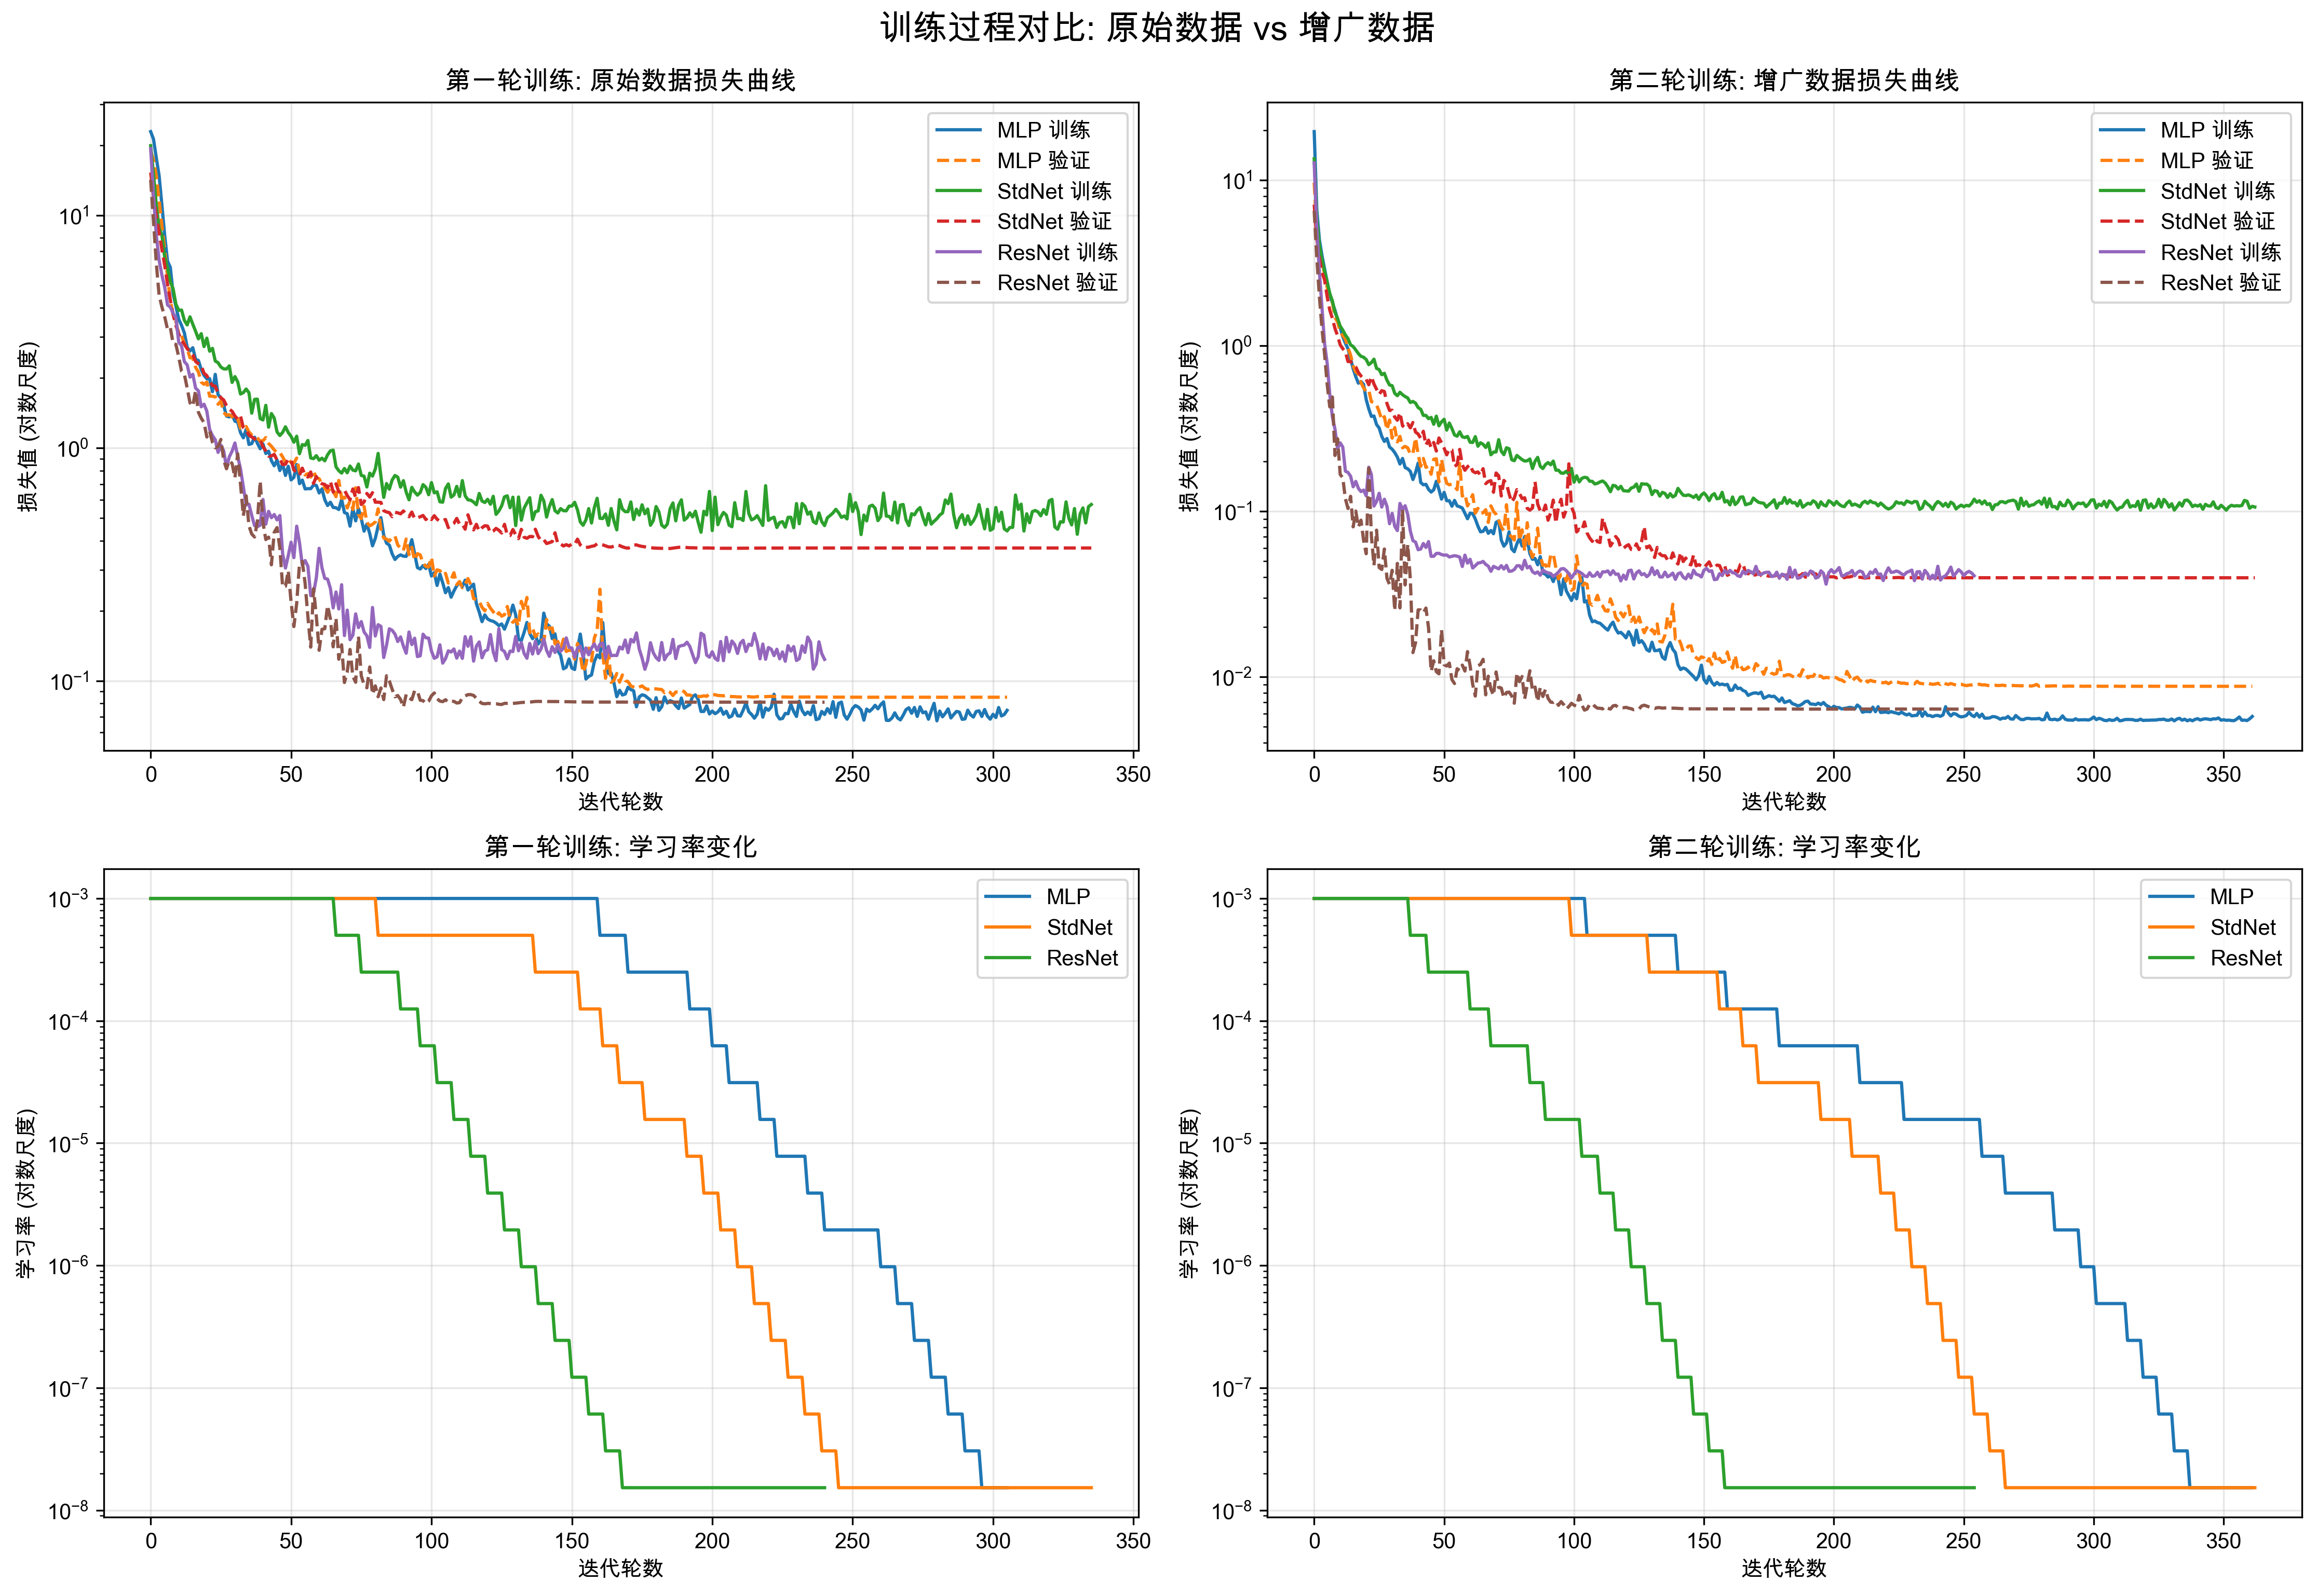
\includegraphics[width=0.9\linewidth]{results_20250330_150206/figures/训练过程对比.png}
    \caption{两阶段训练过程对比(左:原始数据训练,右:增广数据训练)}
    \label{fig:training_process}
\end{figure}

\section{训练结果}
\subsection{训练结果可视化}
参见图\ref{fig:mlp_results}、图\ref{fig:stdnet_results}和图\ref{fig:resnet_results}
\begin{figure}[htbp]
    \centering
    \begin{subfigure}[b]{0.8\textwidth}
        \centering
        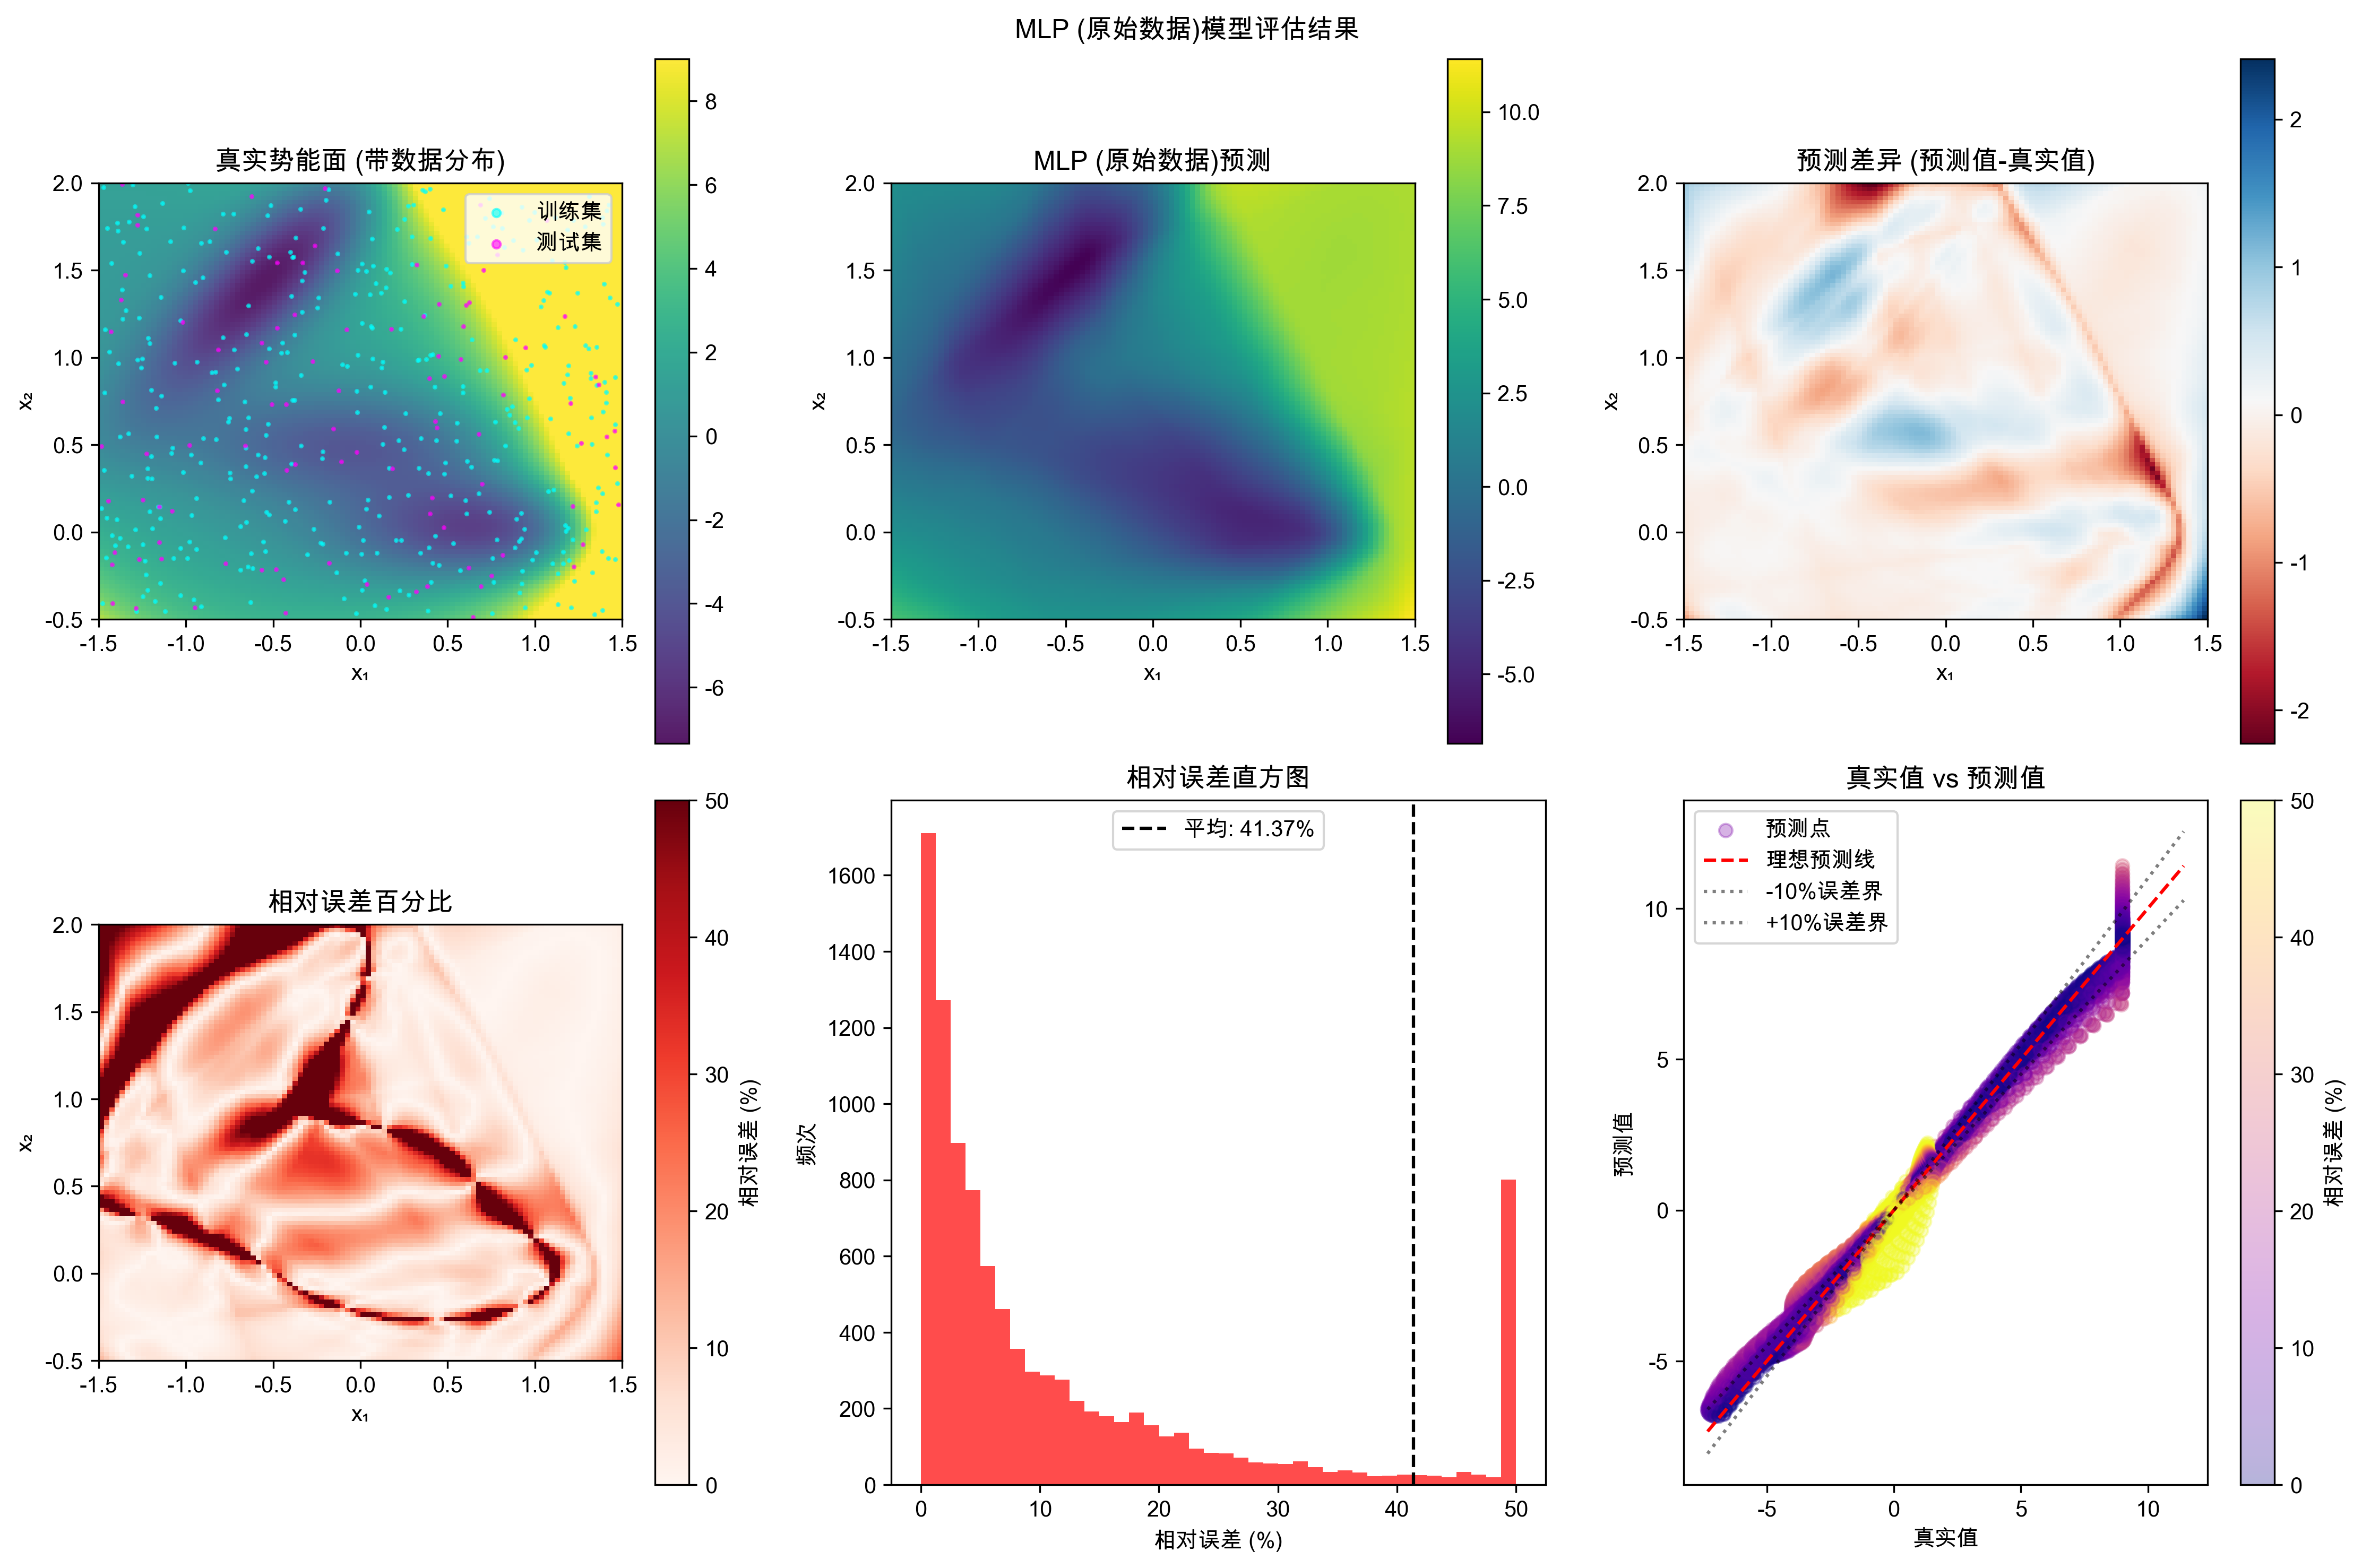
\includegraphics[width=\textwidth]{results_20250330_150206/figures/MLP_round1_评估结果.png}
        \caption{MLP (原始数据)}
        \label{fig:mlp_round1}
    \end{subfigure}

    \vspace{0.5cm}
    \begin{subfigure}[b]{0.8\textwidth}
        \centering
        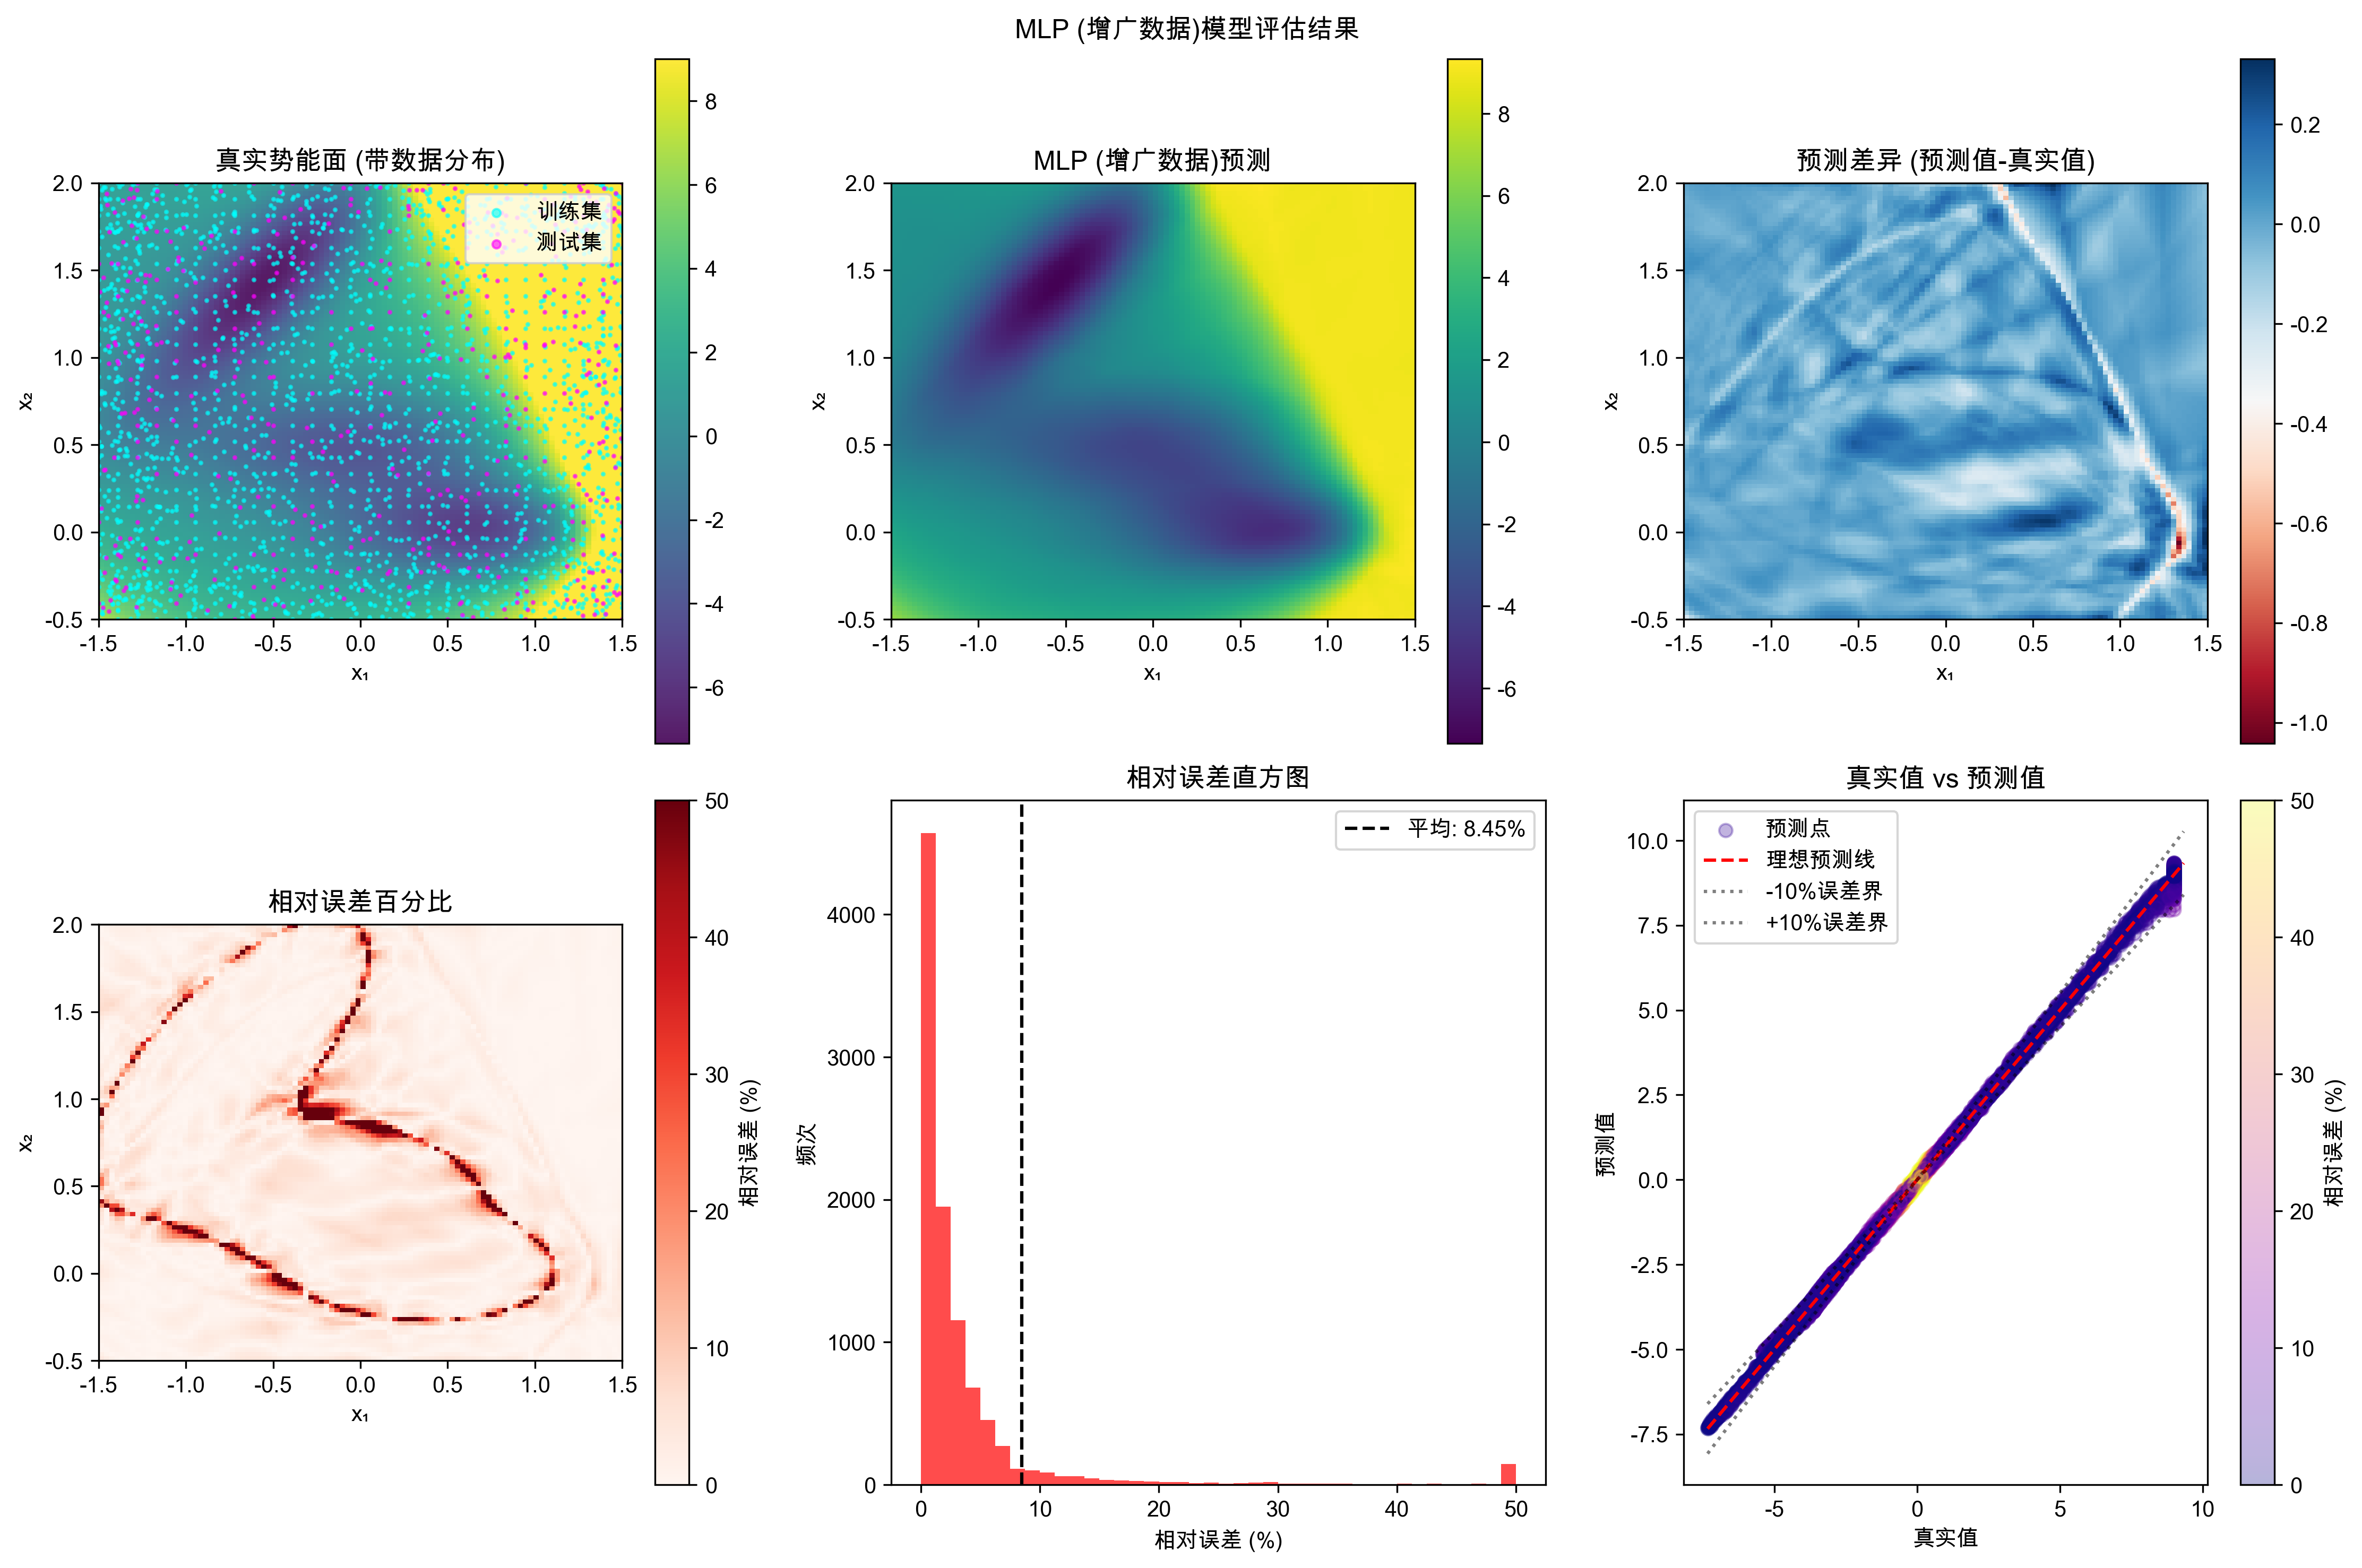
\includegraphics[width=\textwidth]{results_20250330_150206/figures/MLP_round2_评估结果.png}
        \caption{MLP (增广数据)}
        \label{fig:mlp_round2}
    \end{subfigure}
    \caption{MLP模型在原始数据和增广数据上的训练结果对比}
    \label{fig:mlp_results}
\end{figure}

\begin{figure}[htbp]
    \centering
    \begin{subfigure}[b]{0.8\textwidth}
        \centering
        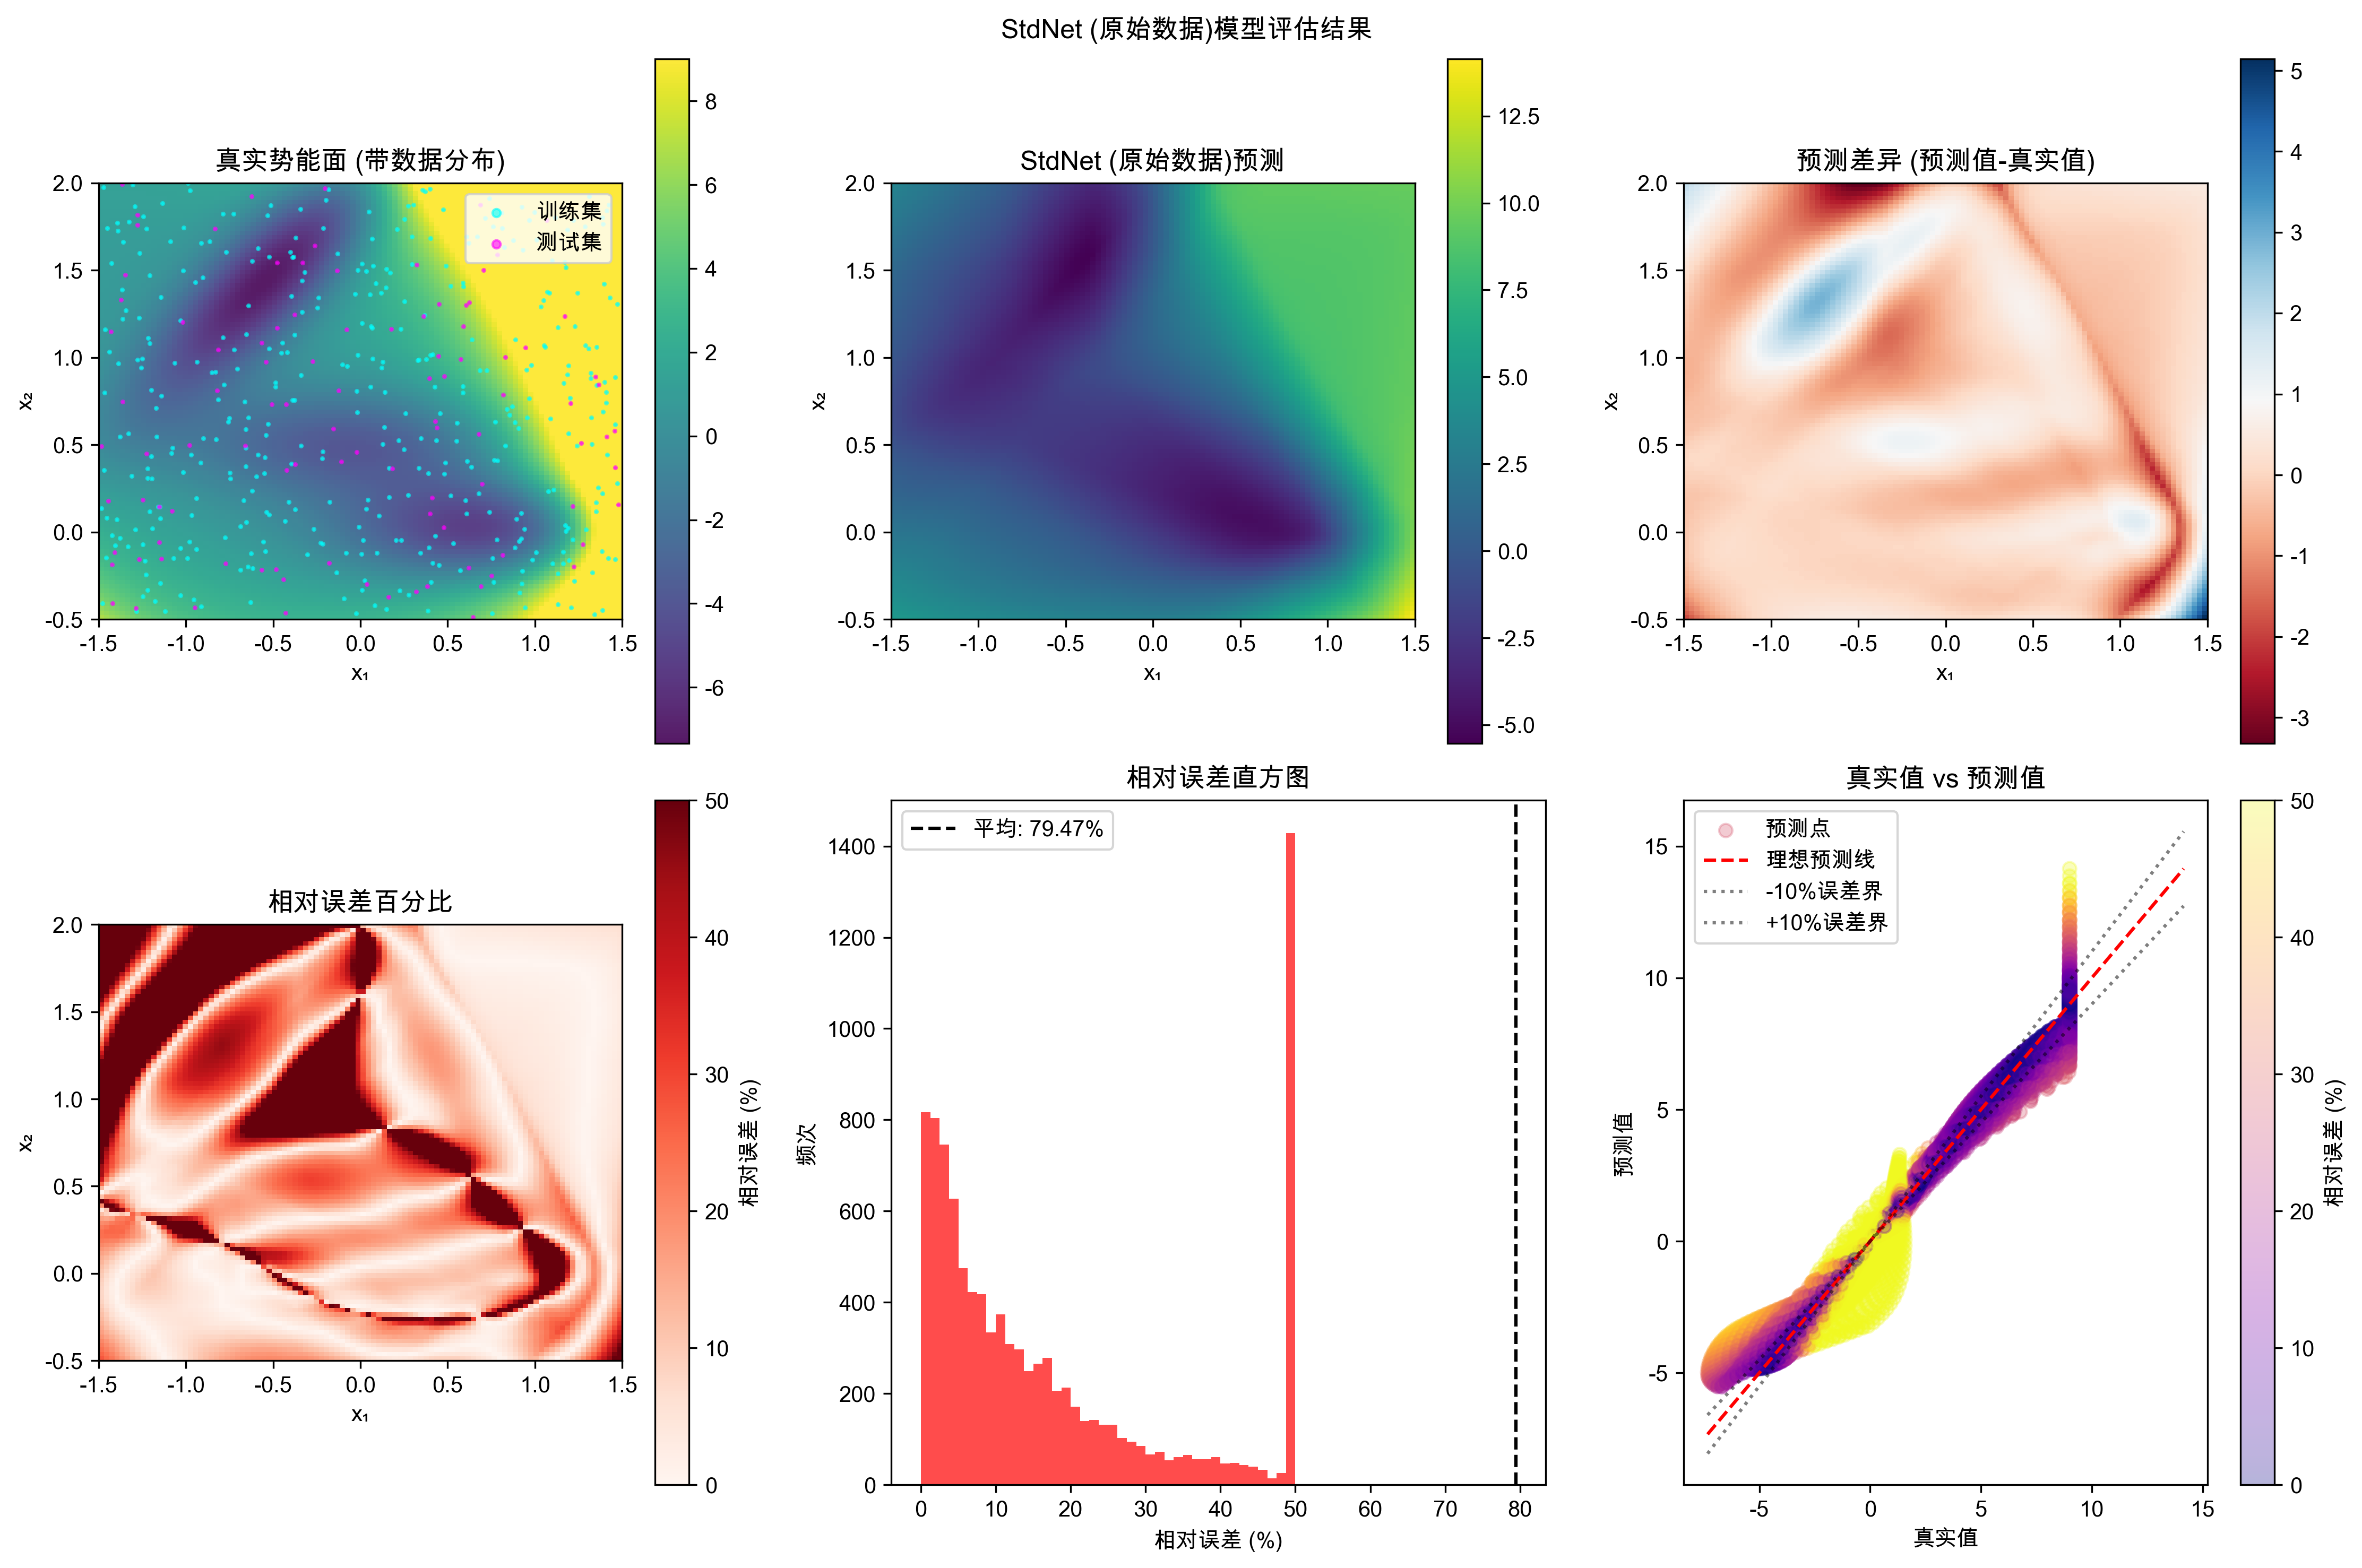
\includegraphics[width=\textwidth]{results_20250330_150206/figures/StdNet_round1_评估结果.png}
        \caption{StdNet (原始数据)}
        \label{fig:stdnet_round1}
    \end{subfigure}

    \vspace{0.5cm}
    \begin{subfigure}[b]{0.8\textwidth}
        \centering
        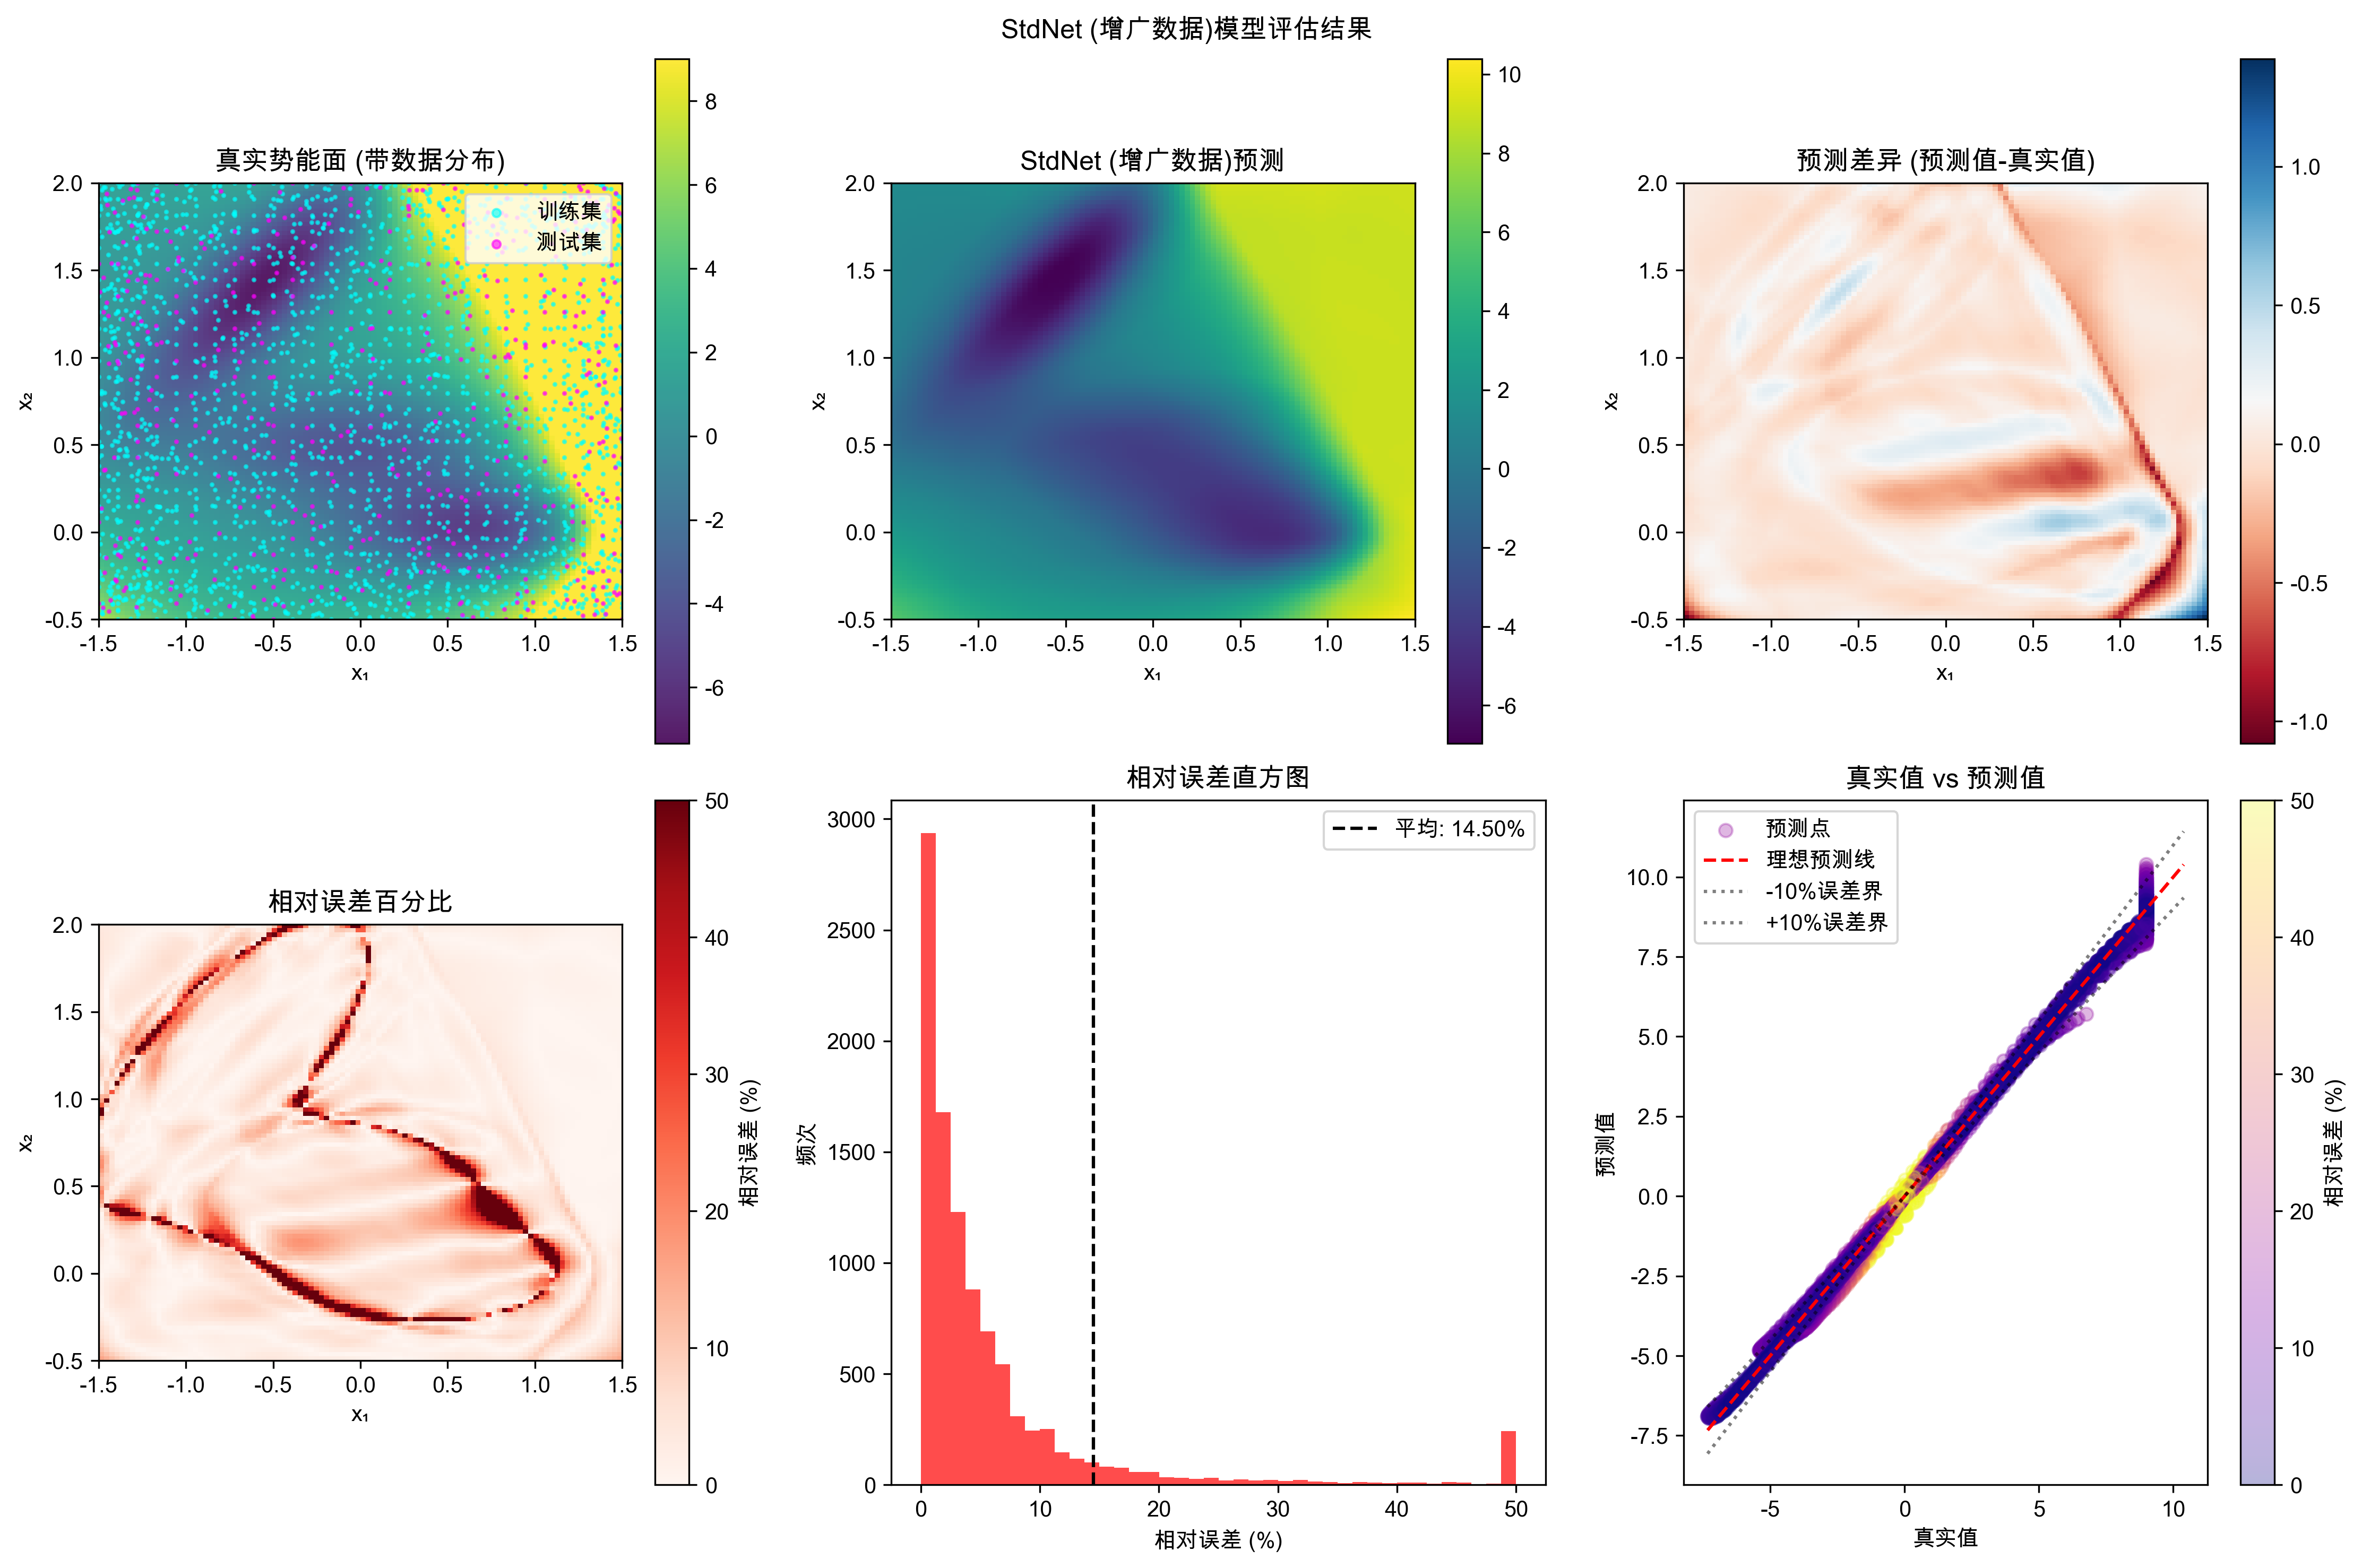
\includegraphics[width=\textwidth]{results_20250330_150206/figures/StdNet_round2_评估结果.png}
        \caption{StdNet (增广数据)}
        \label{fig:stdnet_round2}
    \end{subfigure}
    \caption{StdNet模型在原始数据和增广数据上的训练结果对比}
    \label{fig:stdnet_results}
\end{figure}

\begin{figure}[htbp]
    \centering
    \begin{subfigure}[b]{0.8\textwidth}
        \centering
        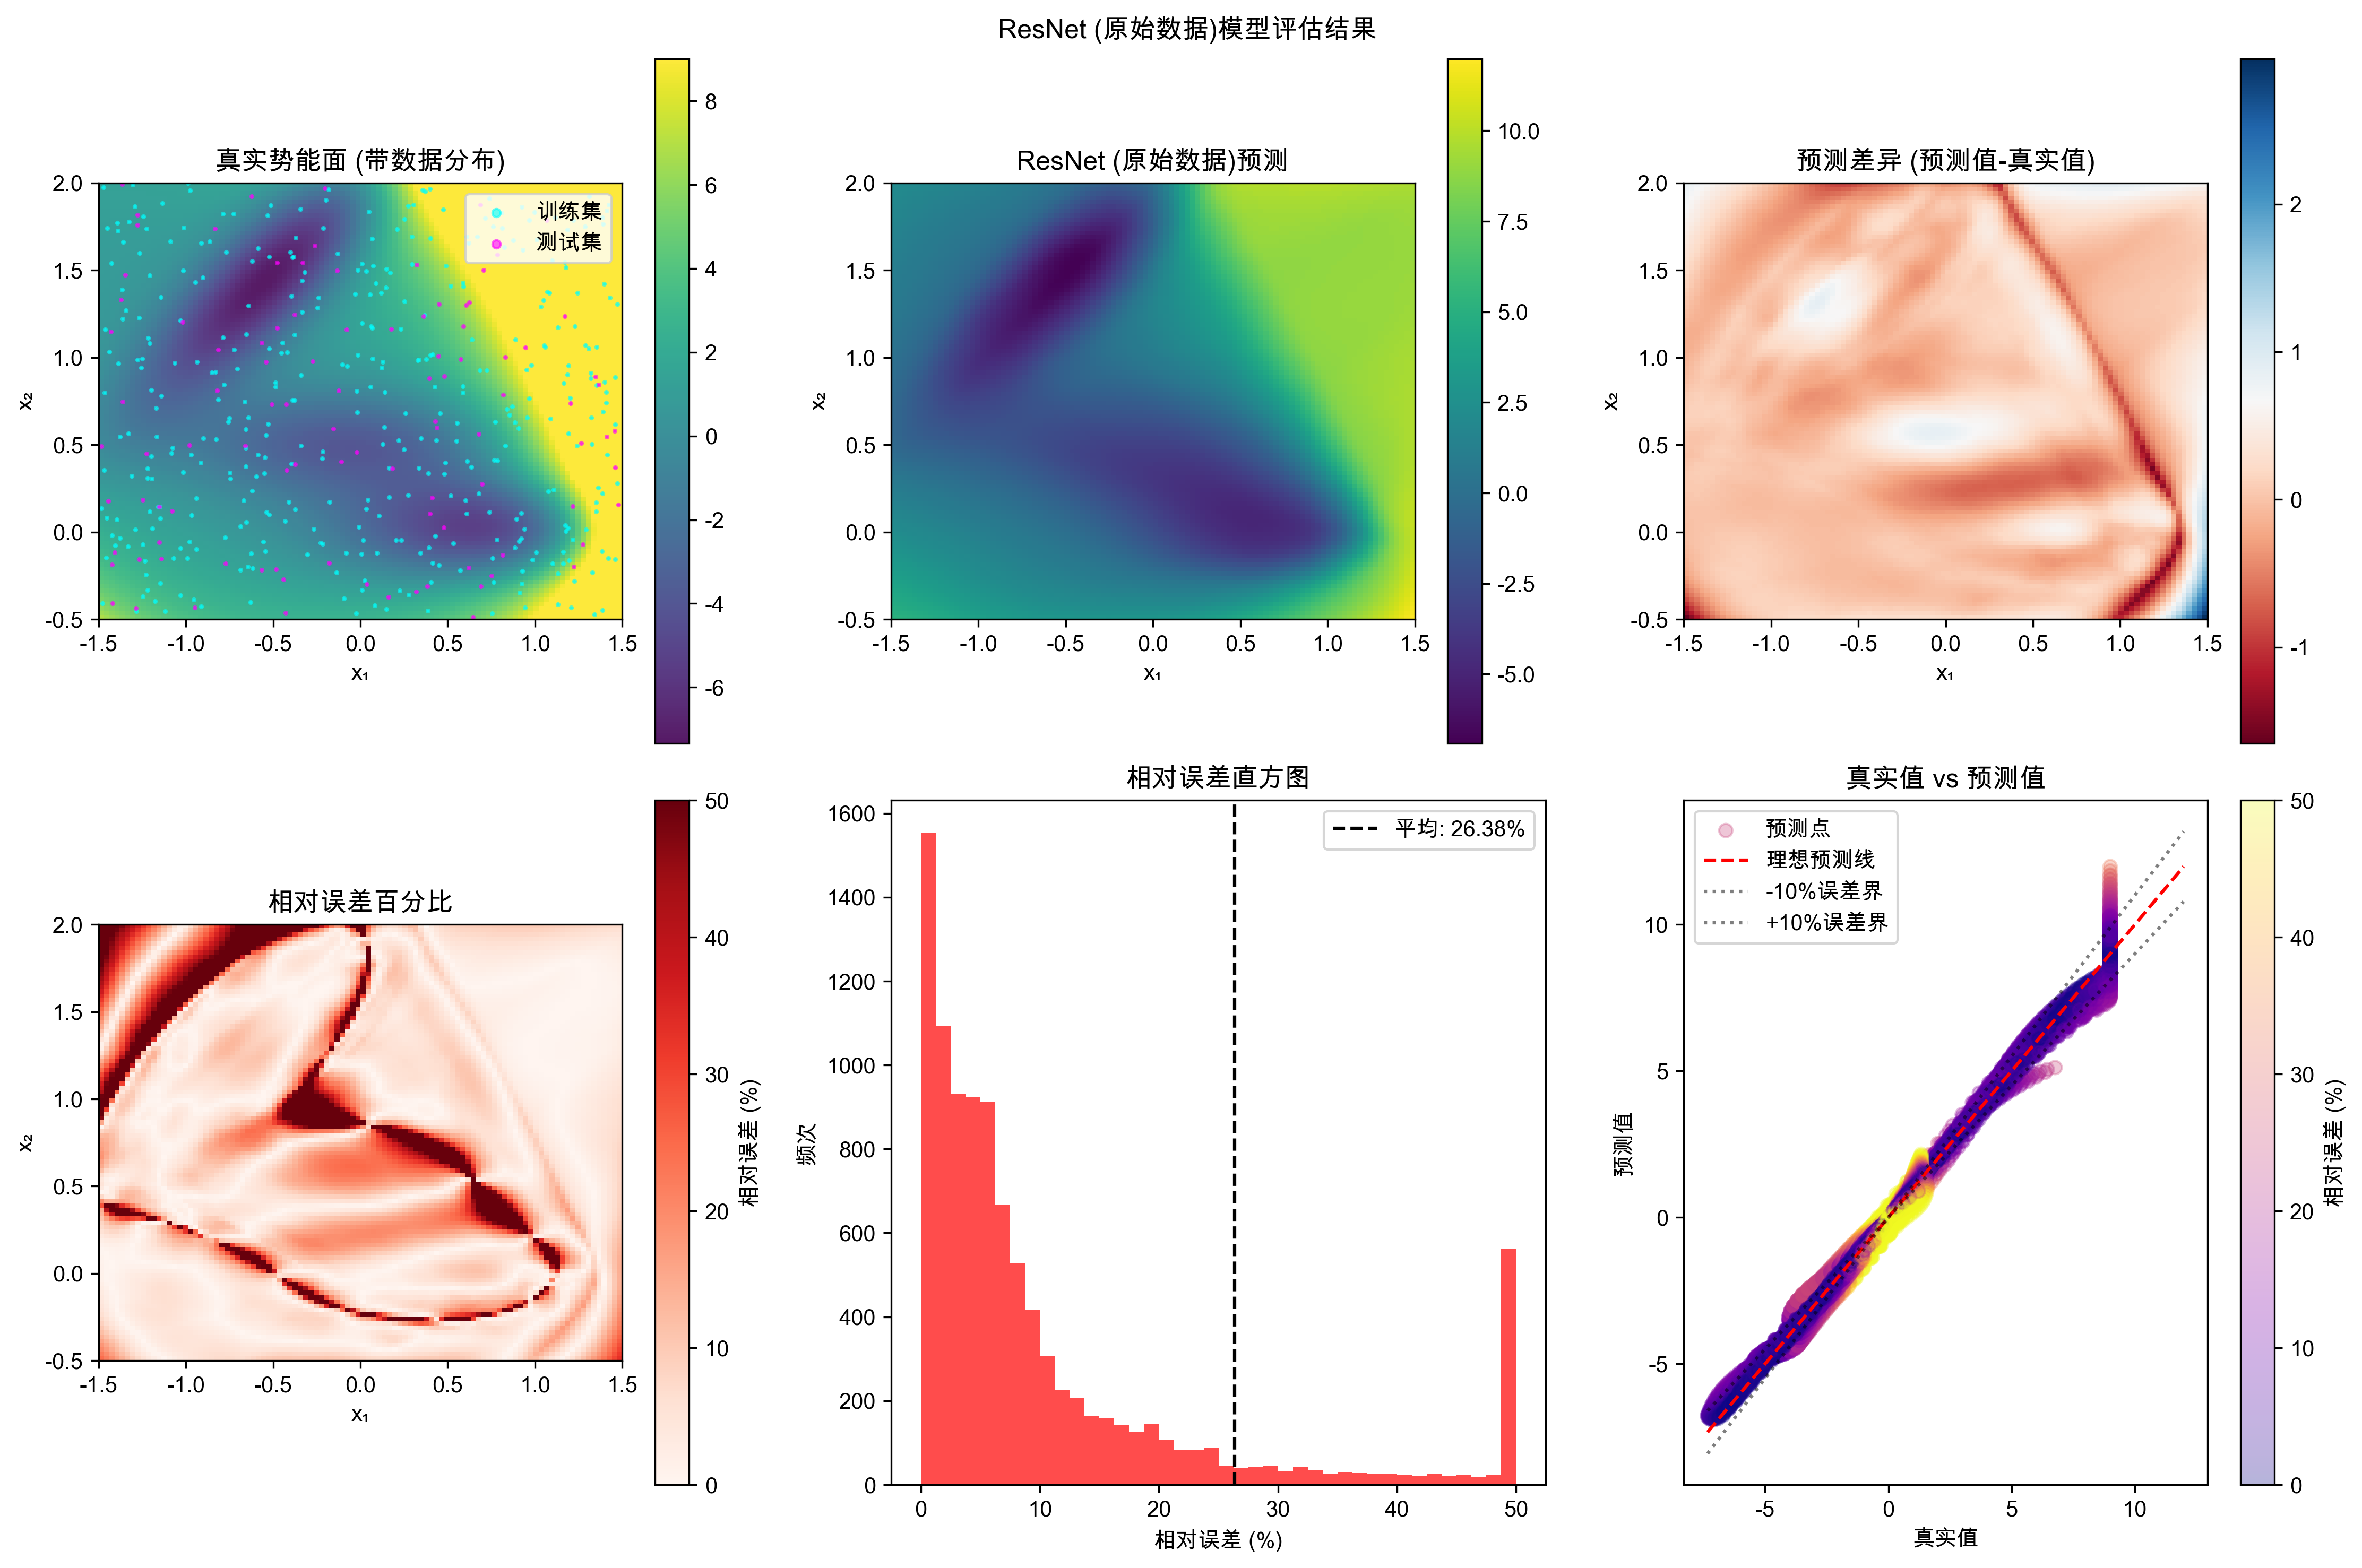
\includegraphics[width=\textwidth]{results_20250330_150206/figures/ResNet_round1_评估结果.png}
        \caption{ResNet (原始数据)}
        \label{fig:resnet_round1}
    \end{subfigure}

    \vspace{0.5cm}
    \begin{subfigure}[b]{0.8\textwidth}
        \centering
        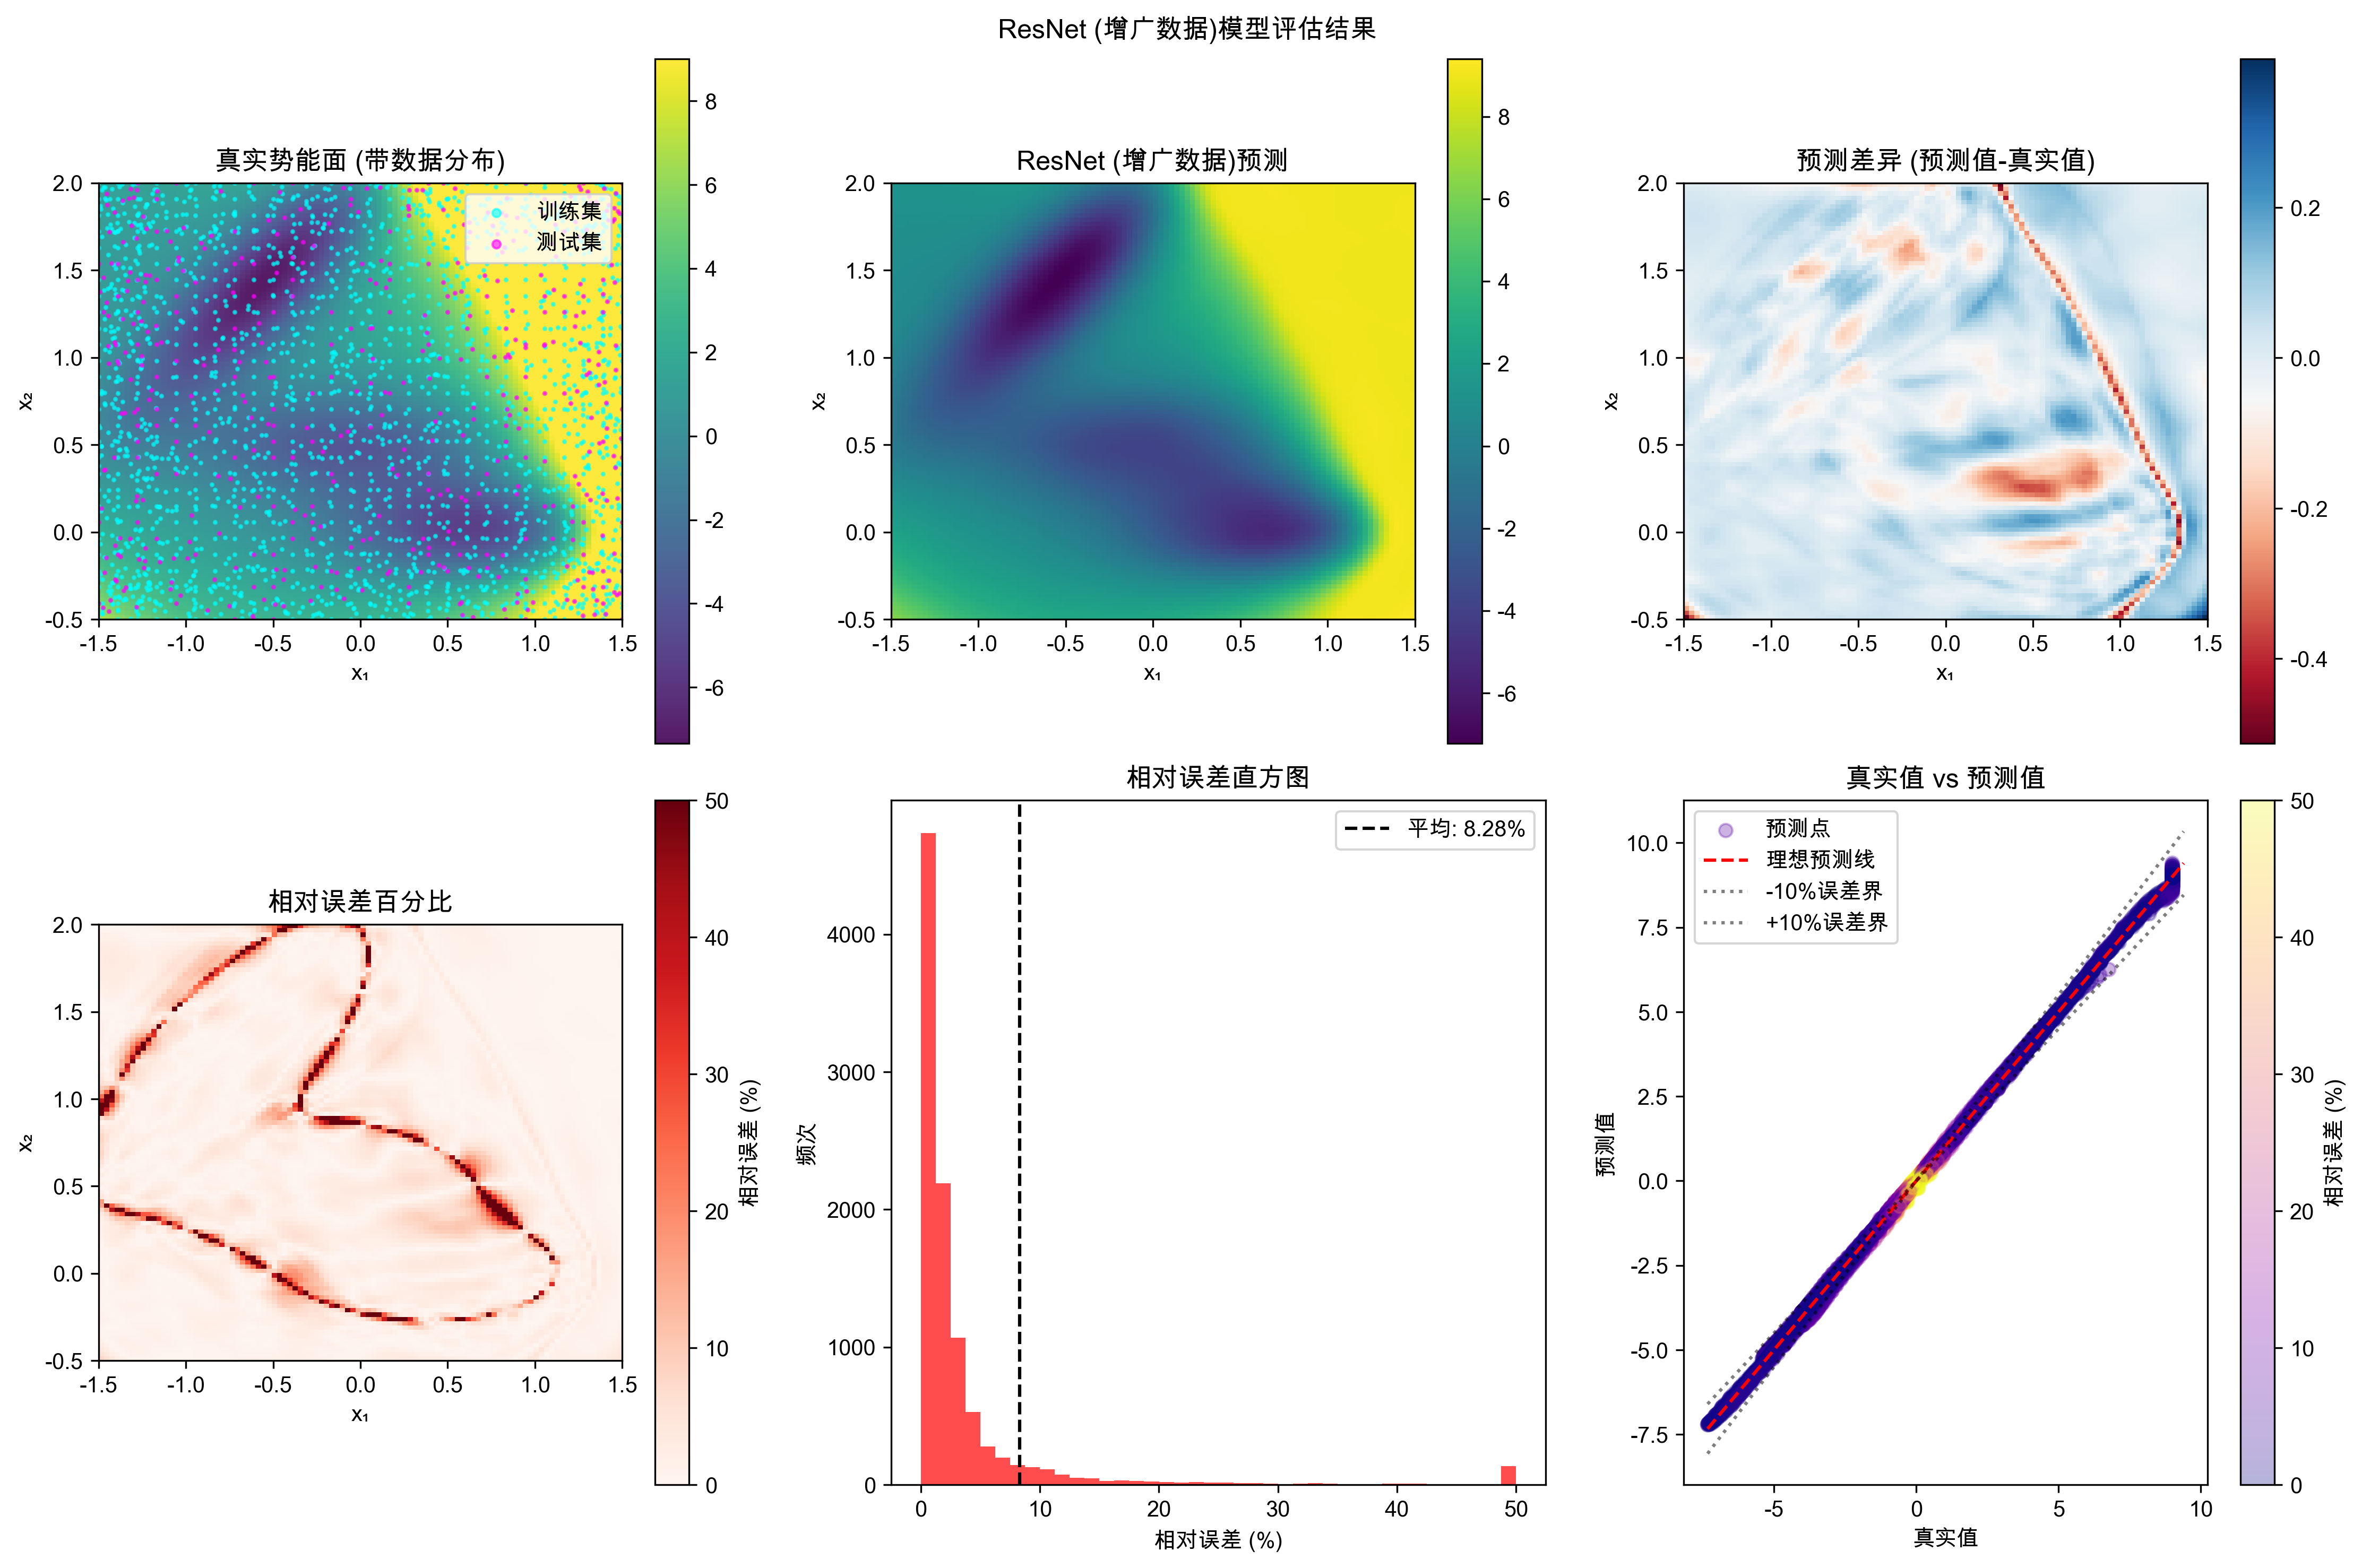
\includegraphics[width=\textwidth]{results_20250330_150206/figures/ResNet_round2_评估结果.png}
        \caption{ResNet (增广数据)}
        \label{fig:resnet_round2}
    \end{subfigure}
    \caption{ResNet模型在原始数据和增广数据上的训练结果对比}
    \label{fig:resnet_results}
\end{figure}

\subsection{结果分析}
从可视化图中可以观察到几个关键现象:

\begin{enumerate}
    \item \textbf{数据增广效果}:所有模型在使用增广数据后,预测精度显著提高,尤其在势能面的边缘区域。

    \item \textbf{误差分布特征}:相对误差主要集中在势能值的过渡区域,而在势能的主要极小值区域(M\"{u}ller-Brown势能的三个主要井区)预测精度较高。

    \item \textbf{相对误差特点}:所有模型的相对误差分布都呈现右偏分布特性,即大多数区域误差较小(分布直方图左侧集中),少数区域存在较大误差(分布直方图右侧拖尾)。
\end{enumerate}

\newpage
\section{模型评估}

\begin{figure}[htbp]
    \centering
    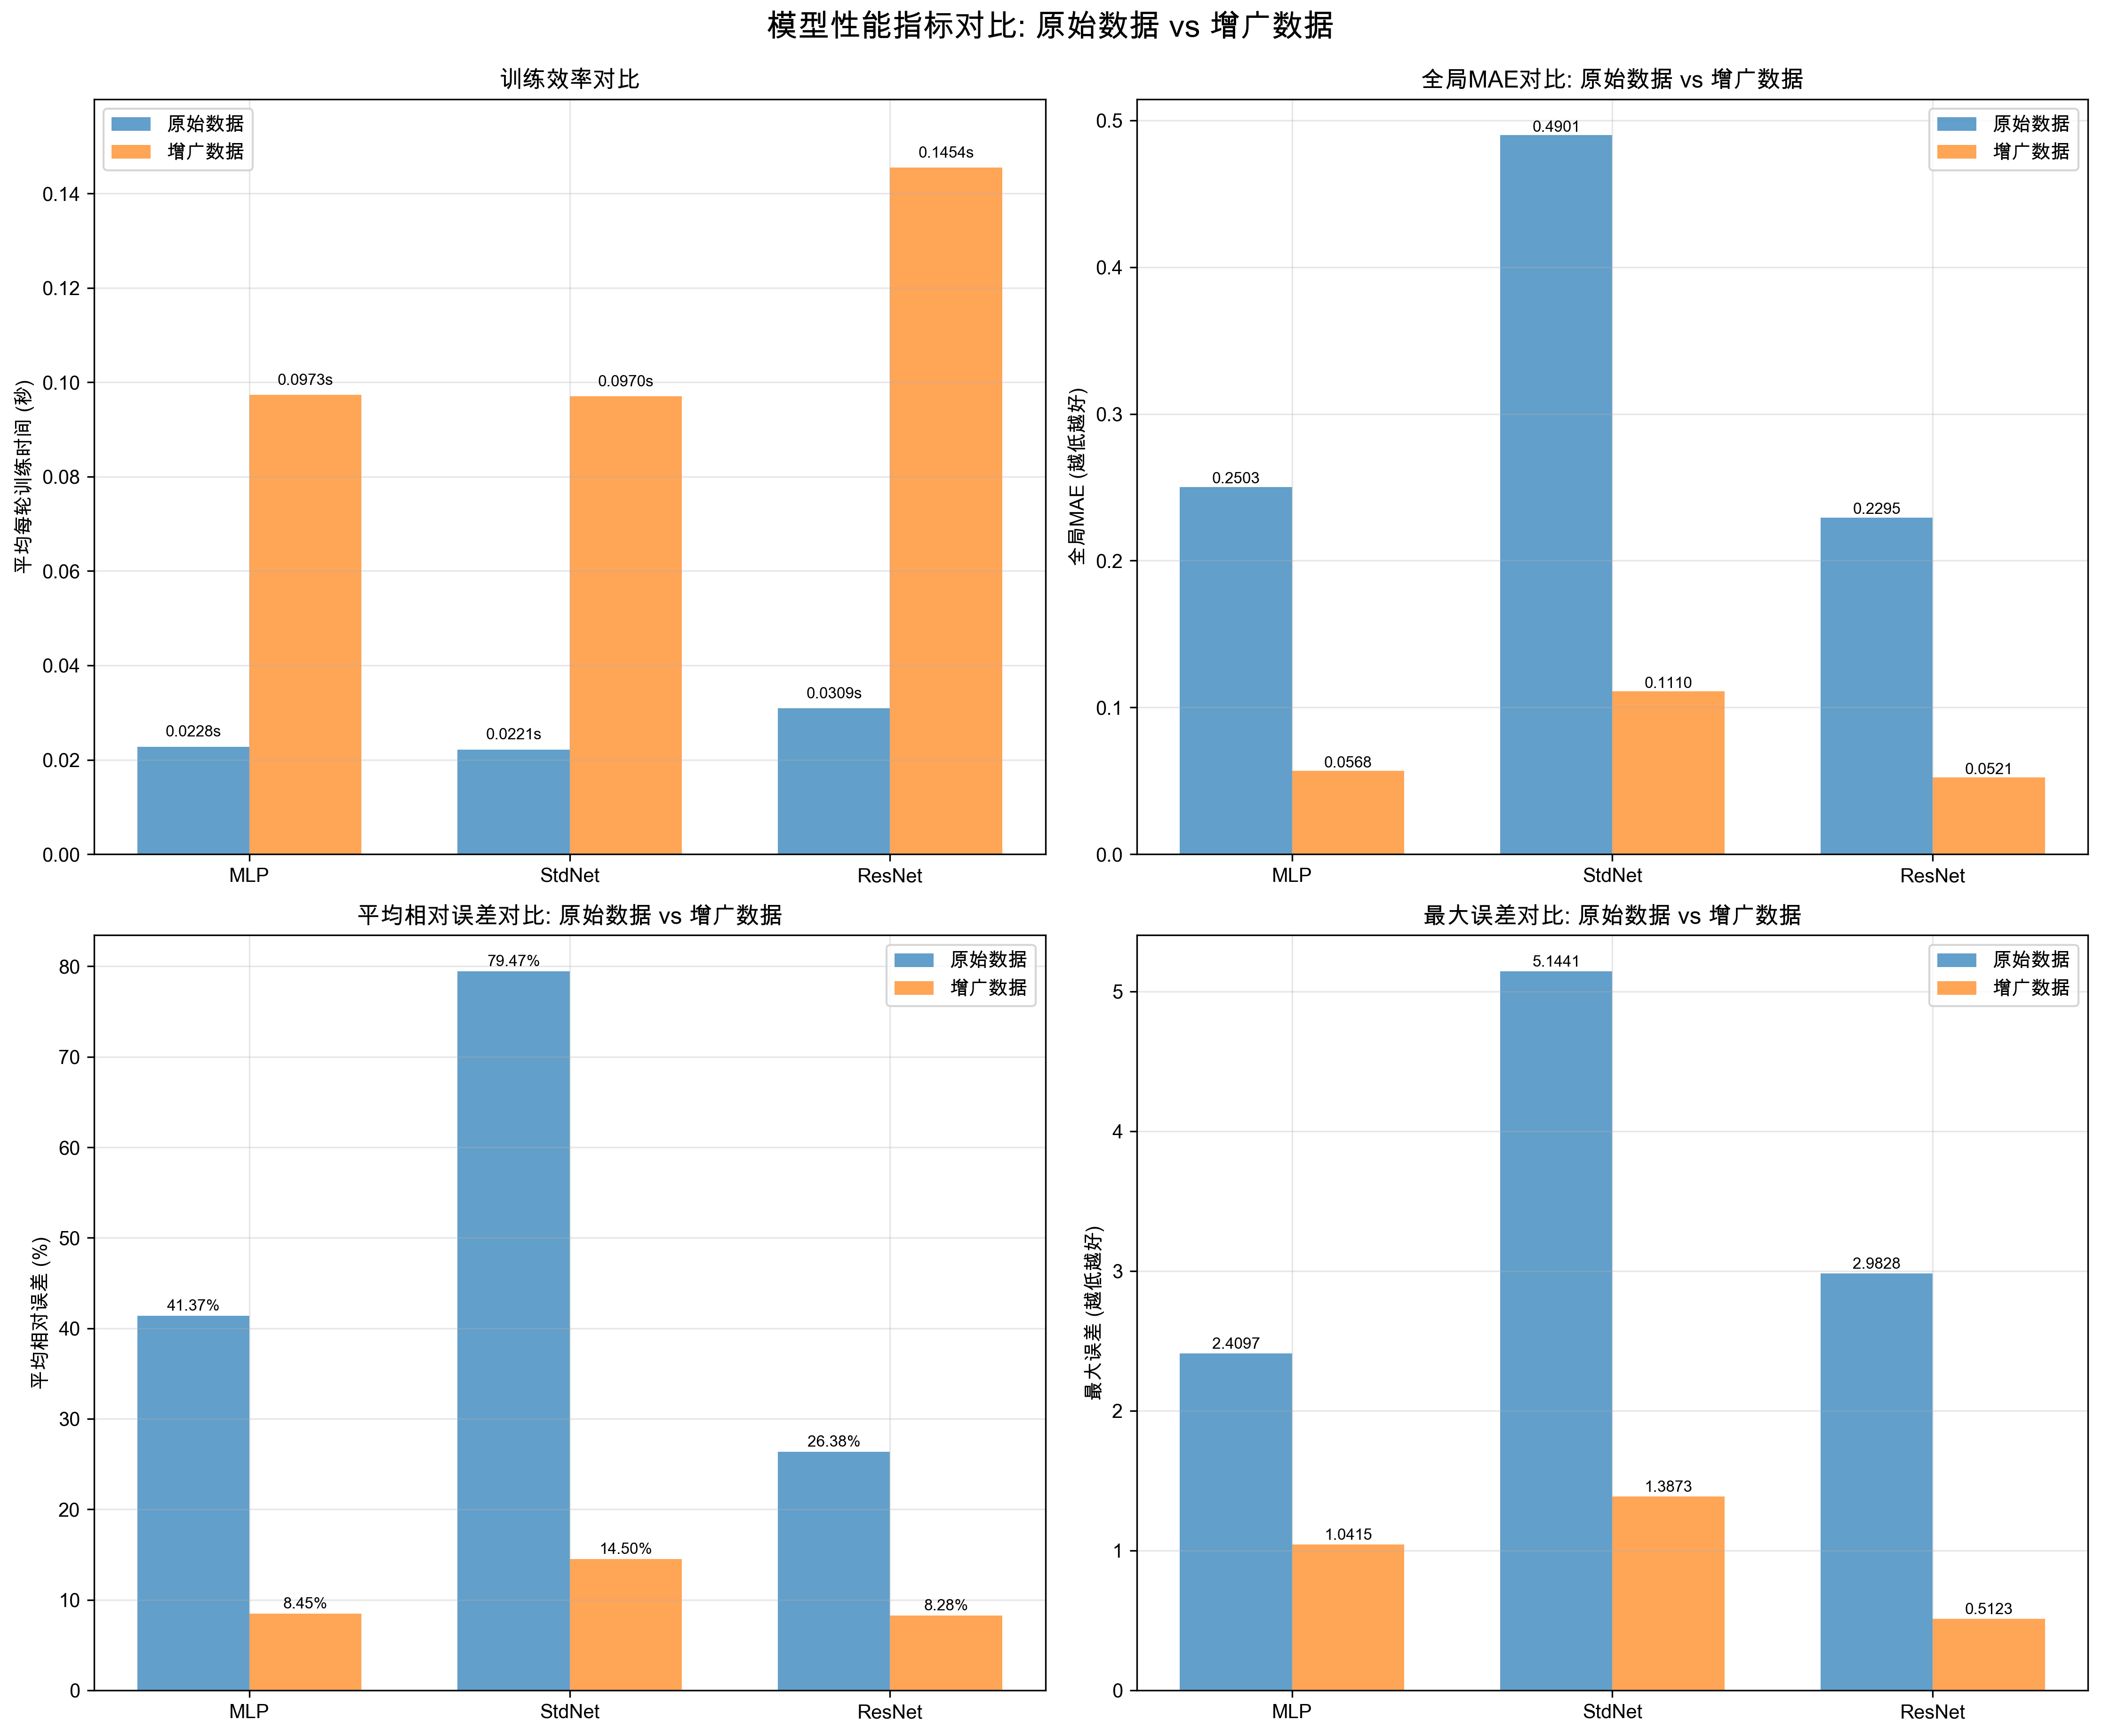
\includegraphics[width=0.9\textwidth]{results_20250330_150206/figures/性能指标对比.png}
    \caption{各模型在原始数据和增广数据上的性能指标对比}
    \label{fig:performance_comparison}
\end{figure}

Scaling Law大展神威,StdNet表现不尽人意。

\newpage
\subsection{详细评估指标}

\begin{table}[htbp]
    \centering
    \caption{模型基本特性对比}
    \label{tab:model_basic}
    \begin{tabular}{lccc}
        \toprule
        \textbf{指标} & \textbf{MLP} & \textbf{StdNet} & \textbf{ResNet} \\
        \midrule
        模型参数量       & 25,217       & 33,793          & 66,561          \\
        标准化层        & 否            & 是               & 是               \\
        Dropout正则化  & 否            & 是               & 是               \\
        残差连接        & 否            & 否               & 是               \\
        \bottomrule
    \end{tabular}
\end{table}

\begin{table}[htbp]
    \centering
    \caption{原始数据上(500点)的训练结果}
    \label{tab:results_round1}
    \begin{tabular}{lccc}
        \toprule
        \textbf{指标} & \textbf{MLP} & \textbf{StdNet} & \textbf{ResNet} \\
        \midrule
        训练轮数        & 306          & 336             & 241             \\
        总训练时间(秒)    & 6.97         & 7.44            & 7.44            \\
        平均每轮时间(秒)   & 0.0228       & 0.0221          & 0.0309          \\
        最终学习率       & 1.53e-08     & 1.53e-08        & 1.53e-08        \\
        全局MAE       & 0.2503       & 0.4901          & 0.2295          \\
        训练集MAE      & 0.1852       & 0.4008          & 0.1774          \\
        测试集MAE      & 0.2095       & 0.4368          & 0.2062          \\
        RMSE        & 0.3793       & 0.7310          & 0.3431          \\
        最大误差        & 2.4097       & 5.1441          & 2.9828          \\
        平均相对误差(\%)  & 41.3736      & 79.4676         & 26.3759         \\
        \bottomrule
    \end{tabular}
\end{table}

\begin{table}[htbp]
    \centering
    \caption{增广数据上(2500点)的训练结果}
    \label{tab:results_round2}
    \begin{tabular}{lccc}
        \toprule
        \textbf{指标} & \textbf{MLP} & \textbf{StdNet} & \textbf{ResNet} \\
        \midrule
        训练轮数        & 362          & 363             & 255             \\
        总训练时间(秒)    & 35.22        & 35.22           & 37.09           \\
        平均每轮时间(秒)   & 0.0973       & 0.0970          & 0.1454          \\
        最终学习率       & 1.53e-08     & 1.53e-08        & 1.53e-08        \\
        全局MAE       & 0.0568       & 0.1110          & 0.0521          \\
        训练集MAE      & 0.0481       & 0.1019          & 0.0452          \\
        测试集MAE      & 0.0578       & 0.1176          & 0.0520          \\
        RMSE        & 0.0874       & 0.1748          & 0.0766          \\
        最大误差        & 1.0415       & 1.3873          & 0.5123          \\
        平均相对误差(\%)  & 8.4511       & 14.4967         & 8.2789          \\
        \bottomrule
    \end{tabular}
\end{table}

\begin{table}[htbp]
    \centering
    \caption{数据增广带来的性能改进}
    \label{tab:improvement}
    \begin{tabular}{lcc}
        \toprule
        \textbf{模型} & \textbf{全局MAE改进} & \textbf{相对误差改进} \\
        \midrule
        MLP         & 77.28\%          & 79.57\%         \\
        StdNet      & 77.35\%          & 81.76\%         \\
        ResNet      & 77.28\%          & 68.61\%         \\
        \bottomrule
    \end{tabular}
\end{table}

\end{document}